\appendix

\addtocontents{toc}{\protect\setcounter{tocdepth}{0}}

\section{Representations}

\subsection{All network features are correlated with one another}\label{sec:bag-of-features-hcp}
The experiment is repeated using the binarized structural connectomes from HCP dataset. For all $1059$ connectomes, which have 70 vertices, the network features are computed. Figure \ref{fig:exp6_hcp} \textit{top row} shows the distributions for all connectomes, and \textit{middle row} and \textit{bottom row} show the distributions after constraining by considering all connectomes with number of edges between $1010$ and $1210$, and then by choosing a network with $1100$ edges at random and choosing all networks with at most $300$ edge differences. Even in real data, constraining the networks produce similar distributions of network statistics. 

\begin{figure}[b!]
    \centering
    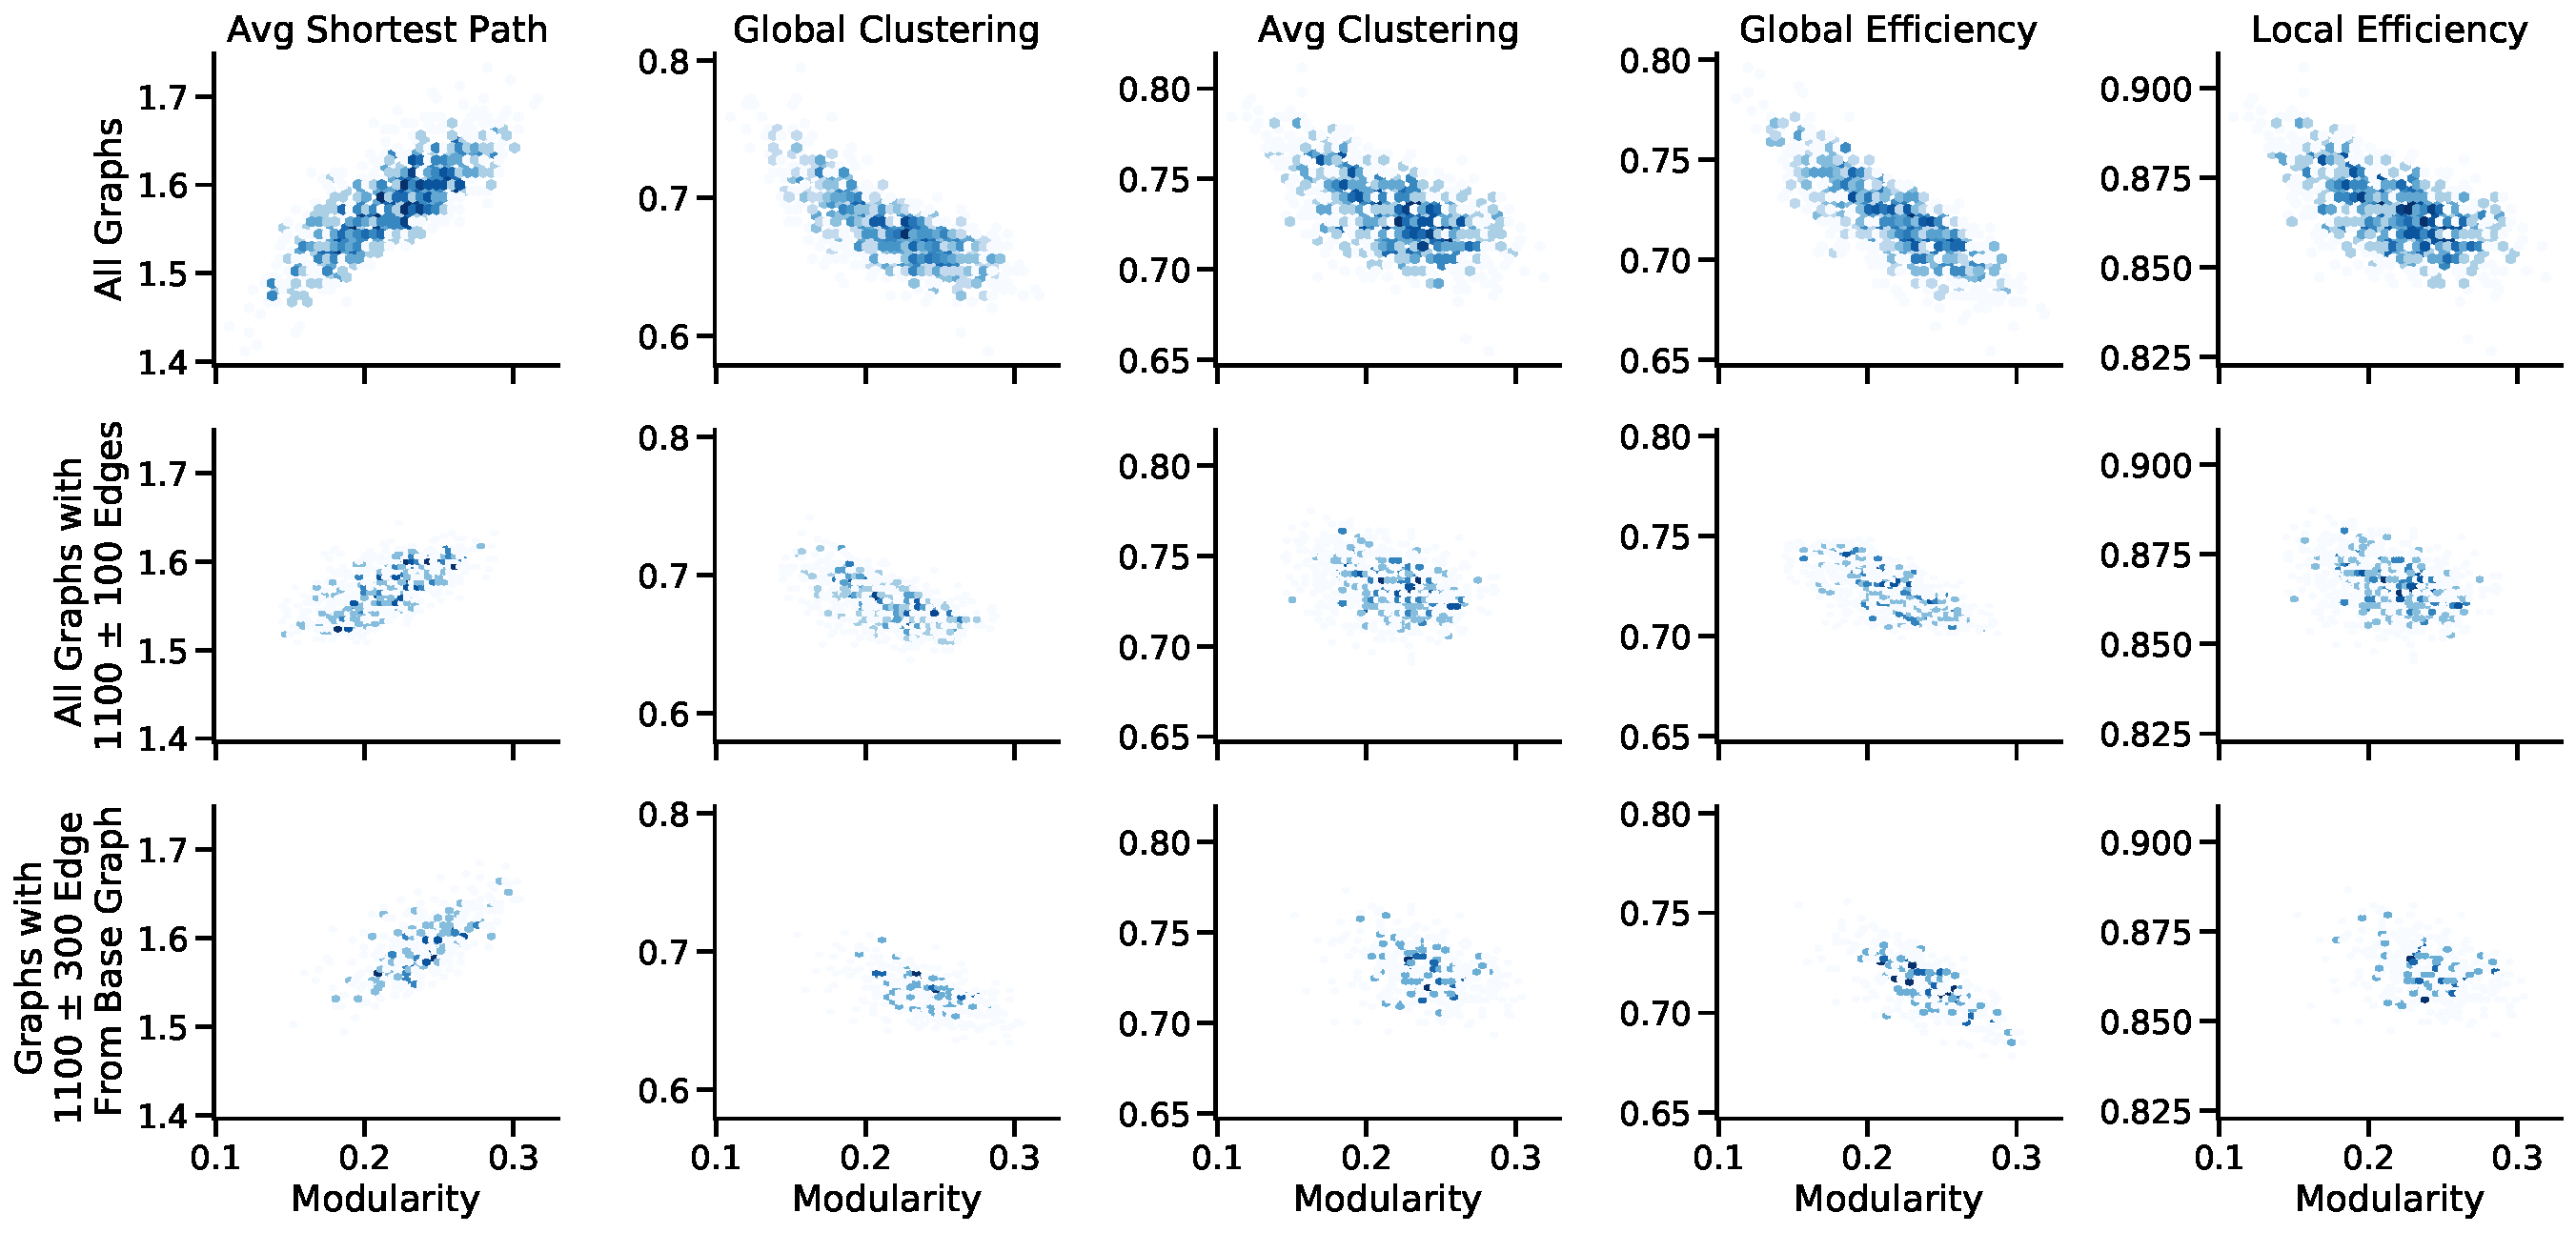
\includegraphics[width=\textwidth]{figures/exp6_hcp.pdf}
    \caption{\textbf{Density plots of network statistics on HCP connectomes.} All connectomes ($N=1059$) have 70 vertices defined by the Deskian parcellation. 
    \textit{(Top row)} The distributions of networks statistics for all HCP connectomes are shown.
    \textit{(Middle Row)} connectomes are constrained by only considering all networks with $1100 \pm 100$ edges.
    and \textit{(Bottom Row)} A base graph with $1100$ edges is chosen at random, and only networks that have differences up to $300$ edges are considered. Similar to the simulated examples, the distributions are qualitatively similar.}
    \label{fig:exp6_hcp}
\end{figure}


\section{Model Extensions}\label{sec:model_extensions}


\subsection{Weighted Models}
% The unweighted graph in Section \ref{sec:unwt_graph} can be extended to the weighted graph model $G = (V, E, w)$, where $V$ and $E$ are the vertices and edges as described previously, and $w : E \rightarrow R$ is a function that assigns a weight to each edge within the graph. Commonly, we are concerned with the case where $R$ is taken to be the non-negative portion of the real line, $[0, \infty)$, and where $E$ is taken to be all possible pairs of vertices $V \times V$. We denote $w_{i,j} \triangleq w(v_i, v_j)$ if $(v_i, v_j) \in E$ for two vertices $v_i, v_j$ which are connected, and $w_{ij} \triangleq 0$ if $v_i, v_j$ are not connected. In this fashion, entries of the adjacency matrix $\A_{ij}$ are taken to be the weights $w_{ij}$ for $i, j \in [n]$. Again, we will take the graphs considered to be undirected; that is, $\A_{ij} = \A_{ji}$ for all $i \neq j$, and with no self-loops; ie, $\textrm{diag}(\A) = \vec 0$. As before, under this specification, the adjacency matrix $\A$ provides a unique representation of $G$.

The single graph models in Section \ref{sec:single_graph_models} can be extended to weighted graphs trivially. For example, in the \textit{a priori} $\sbm$, each distinct community of edges within the graph, simply take the corresponding entries of the adjacency matrix $\A_{ij}$ to take distribution $F_{ij}$ with parameters $\pmb \theta_{ij}$. Adding additional structure to $F_{ij}$ allows the parameters $\theta_{i,j}$ to be estimable for a single graph. In particular, we will be concerned with the Truncated-Normal $\sbm$, where:
\begin{align*}
    \A_{ij}; \vec\tau_i = k, \vec\tau_j = l, \pmb \theta_{kl} \overset{ind}{\sim} \tnorm (\pmb \theta_{kl})
\end{align*}
Where $\pmb \theta_{kl} = (\mu_{k,l}, \sigma^2_{k,l}, \textrm{min}_{k,l}, \textrm{max}_{k,l})$ are the parameters associated with the $k, l$ block of edge weights.

\subsection{Degree-Corrected Models}
In the standard $\sbm$ defined in Section \ref{sec:usbm}, the degree of a vertex, or the expected number of edges incident to a vertex, is constant within each block. Thus, vertices with same block assignment are stochastically equivalent to each other, which can limit practical applications \cite{karrer2011stochastic}. 
In $\mathsf{degree-corrected} \sbm$ ($\dcsbm$),  there is an additional ``promiscuity'' parameter that allows vertices within blocks to have heterogeneous expected degree distributions. 

Similar to the standard $\sbm$, the \textit{a priori} $\dcsbm$ is parameterized by a vertex assignment vector $\vec \tau \in \left\{1, \hdots, K\right\}^n$, a symmetric $K \times K$ block connectivity probability matrix $\B$ with entries in $[0,1]^{K \times K}$, and the degree correction (``promiscuity'') vector $\vec \theta \in\RR^n$. 
The degree correction vector is constrained such that $\sum_i^n \vec \theta_i \mathbb{I} (\tau_i=k)=1$ for $k\in[K]$ where $\mathbb{I}$ is an indicator function. 
The model is $\A\sim\dcsbm_n(\vec\tau, \B, \vec \theta)$ if $\A$ has entries $\A_{ij} \sim \bern(\vec\theta_i \vec\theta_j\B_{kl})$ where $k=\tau_i , l=\tau_j$, for $i, j \in [n]$, and $k, l \in [K]$. 
The \textit{a posteriori} $\dcsbm$ model is additionally parameterized by a block membership probability vector $\vec{\pi} = [\pi_1,\dots,\pi_K]^\top$. The model is $\A \sim \sbm_n(\vec \pi,\B, \vec \theta)$ if $\A$ has entries $\A_{ij} \big | k=\tau_i, l=\tau_j \sim \bern(\vec\theta_i \vec\theta_j\B_{kl})$, where $\tau_i {\sim} \multinomial(\vec \pi)$ for $i \in [n]$. 


% 7. theory
%     1. single graph theory
%         a. "you say i say"
%         b. central limit theorem for ase/lse
%     2. multi graph theory 
%         a. mase/omni
%         c. nonpar + semipar theory
%         d. sgm correlated-SBM/ER theory

\section{Theory for Statistical Models}
In this section, we provide general outlines of the theorems and proofs for statistical models in Section \ref{sec:models} and algorithms in Section \ref{sec:algorithms}.

\subsection{Theory for Single Graph Models}\label{sec:theory_single}

Graph features, such as the ones described in Section~\ref{sec:bag-of-features}, are popularly used to test hypothesis about a graph. However,  the distribution of such features is usually unknown, and even in cases where the asymptotic distribution is available, one needs to proceed with caution as some of the asymptotic results might be misleading \cite{priebe2010you}.  \cite{Rukhin2010} studies the behavior of two simple graph features, namely, the number of edges and the maximum  degree, for testing a simple hypothesis question about the distribution of a graph. While the statistic based on the number of edges achieves a higher power in the limit as the number of vertices grows, a comparative power analysis shows that even for large graphs with $n\leq 10^{24}$, the statistic based on the maximum degree dominates under certain cases.

A body of existing results in statistical inference for spectral embeddings is reviewed more deeply in \cite{athreya2017statistical}. We summarize next some of the main results related to the exposition in this paper. 
In this section, we assume that a sequence of random adjacency  matrices $\{\A_n, n\geq 1\}$ generated from a sequence of latent positions $\{\X_n, n\geq 1\}$, where  $\A_n\sim \rdpg(\X_n)$, $n\geq 1$ is the adjacency matrix of a graph with $n$ vertices, and $\X_n\in\RR^{n\times d}$ are $d$-dimensional latent positions. We write $(\X_n)_i$ to represent the $i$-th row of $\X_n$, and we assume that the rows of $\X_n$, which correspond to the latent positions, are an i.i.d. sample $(\X_1), \ldots, (\X_n)_n\overset{\text{i.i.d.}}{\sim} F$, where $F$ is a distribution with support $\mathcal{X}\subset\RR^d$. We also  assume that the second moment matrix $\mathbf{\Delta} = \mathbb{E}[(\X_n)_1(\X_n)_1^\top]\in\Real^{d\times d}$, has non-zero eigenvalues.   We use $\widehat{\X}_n=\ase(\A_n)\in\Real^{n\times d}$ to denote the $d$-dimensional adjacency spectral embedding of $\A_n$, and $\widetilde{\X}_n = \lse(\A_n)$  to denote its $d$-dimensional Laplacian spectral embedding.


The adjacency spectral embedding ($\ase$) method described in Section~\ref{sec:ase} is a consistent and asymptotically normal estimator for the latent positions of a random dot product graph. In \cite{sussman2012consistent}, it is shown that clustering rows of the $\ase$ of $\A_n$ can consistently recover the communities of an $\sbm$. Consistency of the latent positions for an $\rdpg$ is studied in  \cite{Sussman2014-zq,Lyzinski2014-pe,Lyzinski2017-cq}. In particular, Theorem 5 of  \cite{Lyzinski2017-cq} shows that with probability tending to one, there exists some orthogonal rotation $\W_n\in\Real^{d\times d}$ such that 
\begin{equation*}
    \max_{i\in[n]}\|(\widehat{\X}_n)_i - \W_n(\X_n)_i\| \leq \frac{Cd^{1/2}\log^2 n}{\sqrt{n}}, \label{eq:thm-ASE-const}
\end{equation*}
where $C>0$ is a constant, and hence, the rows of of $\hat{\X}_n$ converge to the rows of $\X_n$, up to some orthogonal rotation, as the number of vertices $n$ grows. 


Distributional results on the rows of the adjacency spectral embedding show that the error in estimating the true latent positions is asymptotically normally distributed. In particular \cite{Athreya2016} showed  a central limit theorem for the rows of the $\ase$ of $\A_n$, in which the latent positions are shown to converge to a mixture of standard multivariate normal distributions, that is, for any $\mathbf{z}\in\RR^{d}$,
\begin{equation}
   \lim_{n\rightarrow\infty} \mathbb{P}\left(\sqrt{n}\left(\widehat{\X}_n\W_n - \X\right)_i\leq \mathbf{z} \right) = \int_{\mathcal{X}}\Phi(\mathbf{z}, \mathbf{\Sigma}(\mathbf{x}))\  dF(\mathbf{x}),\label{eq:thm-ASE-CLT}
\end{equation}
where $\Phi(\mathbf{z}, \mathbf{\Sigma}(\mathbf{x}))$ is the cumulative distribution function of a multivariate normal distribution with mean zero and a covariance matrix $\mathbf{\Sigma}(\mathbf{x})\in\Real^{d\times d}$ that is a function of $\mathbf{x}\in\mathcal{X}$ (see \cite{Athreya2016}, Theorem 1, for an expression of this covariance matrix). 

Similar results to the ones presented above are also available for the Laplacian spectral embedding ($\lse$). In particular, Theorem 3.1 of \cite{tang2018limit} provides an an asymptotic result on the estimation error of the rows of $\widetilde{\X}_n$  with respect to its population version, and Theorem 3.2 shows an analogous result to the one presented in Equation~\eqref{eq:thm-ASE-CLT} to establish the asymptotic normality of the rows of this estimator, that is,
\begin{equation*}
   \lim_{n\rightarrow\infty} \mathbb{P}\left\{\sqrt{n}\left(\W_n(\widetilde{\X}_n)_i - \frac{(\X_n)_i}{\sqrt{\sum_{j}(\X_n)_i^\top (\X_n)_j }} \right)\leq \mathbf{z}\right\}  = \int_{\mathcal{X}}\Phi(\mathbf{z}, \widetilde{\mathbf{\Sigma}}(\mathbf{x}))\  dF(\mathbf{x}),\label{eq:thm-LSE-CLT}
\end{equation*}
for some covariance matrix $\widetilde{\mathbf{\Sigma}}(\mathbf{x})$ which its exact form is presented in \cite{tang2018limit}.

The consistency and asymptotic normality of  $\ase$ and $\lse$ considered in this section  have been recently extended to the $\grdpg$ model  (see Theorems 5-8 in  \cite{rubin2017statistical}). 



\subsection{Theory for Multiple Graph Models}

\subsubsection{Spectral Embeddings}\label{sec:theory_multi}

The results discussed before have been used to develop valid statistical tests for   two-graph hypothesis testing questions. The work of \cite{tang2017semiparametric} studies a semiparametric graph hypothesis testing for the equivalence between the latent positions of the vertices of a pair of graphs. Formally, for each fixed $n$ let $\X_n, \Y_n\in\Real^{n\times d}$ be a sequence of latent positions matrices, and define
$\A_n\sim\rdpg(\X_n)$, $\B_n\sim\rdpg(Y_n)$ as independent random adjacency matrices. The problem of testing the equality of the distributions of $\A_n$ and $\B_n$  is defined as
\begin{equation*}
    \mathcal{H}^n_0:\X_n =_{\W} \Y_n\quad\quad\quad \text{ vs.}\quad\quad\quad \mathcal{H}^n_a:\X_n \neq_{\W} \Y_n,
\end{equation*}
where $\X_n =_{\W}\Y_n$ denotes that $\X_n$ and $\Y_n$ are equivalent up to an orthogonal transformation $\W\in\mathcal{O}_d$, and $\mathcal{O}_d$ is the set of $d\times d$ orthogonal matrices. To define the test statistic, denote  $\widehat{\X}_n = \ase(\A_n)$, $\widehat{\Y}_n=\ase(\B_n)$, and for a matrix $\A\in\Real^{n\times n}$ with singular values $\sigma_1(\A) \geq \ldots\geq \sigma_n(\A)\geq 0$ and largest observed degree $\delta(\A) = \max_{i\in[n]}\sum_{j=1}^n\A_{ij}$, define 
$$\gamma(\A):=\frac{\sigma_d(\A) - \sigma_{d+1}(\A)}{\delta(\A)}.$$ 
Define $T_n$ as the test statistic
\begin{equation*}
    T_n : = \frac{\min_{\W\in\mathcal{O}_d} \|\widehat{\X}_n\W - \widehat{\Y}_n\|_F}{\sqrt{d\gamma^{-1}(\A_n)} + \sqrt{d\gamma^{-1}(\B_n)}}.
\end{equation*}
It is shown in Theorem 3.1 of \cite{tang2017semiparametric} that  $T_n$ is a consistent test for the  hypothesis testing problem described above, in the sense that for any significance level $\alpha$ and $C>1$, then  $\mathbb{P}(T_n> C)\leq \alpha$ for $n$ sufficiently large under $\mathcal{H}^n_0$ (type I error control), and if $\lim_{n\rightarrow\infty}\min_{\W\in\mathcal{O}_d} \|\widehat{\X}_n\W - \widehat{\Y}_n\|_F=\infty$, then $\mathbb{P}(T_n> C)\rightarrow 1$ under $\mathcal{H}^n_a$ (i.e., the type II error vanishes). For specific assumptions and some extensions to other hypothesis testing problems, the reader is referred to \cite{tang2017semiparametric} and \cite{athreya2017statistical}.

When the vertices of the graphs are not necessarily aligned (including cases in which the graphs do not have the same number of vertices), testing equality of latent positions is inappropriate. The work of \cite{tang2017nonparametric} proposes a nonparametric test to determine whether the distribution of the latent positions of the graphs is the same. For a pair of matrices $\X_n\in\Real^{n\times d}$ and $\Y_m\in\real^{m\times d}$ with their rows distributed as $(\X_n)_i\overset{\text{i.i.d.}}{\sim} F$ and $(\Y_m)_i\overset{\text{i.i.d.}}{\sim} G$ and a pair of independent adjacency matrices $\A_n\sim\rdpg(\X_n)$, $\B_n\sim\rdpg(\Y_n)$ , the nonparametric graph hypothesis testing problem is given by
\begin{equation*}
    \mathcal{H}^n_0:F \upVdash G \quad\quad\quad \text{ vs.}\quad\quad\quad \mathcal{H}^n_a: F \nupVdash G,
\end{equation*}
where $F\upVdash G$ indicates equality of the distributions up to an orthogonal transformation. To test such hypothesis, \cite{tang2017nonparametric} proposes to use the following test statistic
\begin{align*}
    U_{n,m}(\X, \Y)=& \frac{1}{n(n-1)}\sum_{j\neq i}\kappa(X_i, X_j)-\frac{2}{mn}\sum_{i=1}^n\sum_{k=1}^m\kappa(X_i, Y_k)\\
    & + \frac{1}{m(m-1)}\sum_{l\neq k}\kappa(Y_k, Y_l),
\end{align*}
where $\kappa:\mathcal{X}\times \mathcal{X}\rightarrow\Real$ is a positive definite kernel. In \cite{tang2017nonparametric}, Theorem 1, it is shown that $U_{n,m}(\X, \Y)$ is a consistent and unbiased estimate of the maximum mean discrepancy \cite{gretton2012kernel} between the distributions $F$ and $G$. Furthermore, under the null hypothesis, the quantity $(m+n)U_{n,m}(\X, \Y)$ converges in distribution to an infinite weighted sum of independent chi-squared random variables as $n,m\rightarrow \infty$, provided that $\frac{n}{n+m}\rightarrow \rho \in (0, 1)$.  Moreover, when the latent positions are used in place of the true latent positions, then Theorem 4 of \cite{tang2017nonparametric} shows that the difference between $U_{n,m}(\widehat{\X}, \widehat{\Y})$  and $U_{n,m}(\X, Y)$ converges to zero sufficiently fast to yield a consistent test procedure.

% Under the null hypothesis that $F = G$ (up to some orthogonal transformations), 
% \begin{equation*}
%     (m+n)(U_{n,m}(\widehat{\X}, \widehat{\Y}) - U_{n,m}({\X}, {\Y}\W_{n,m})) \overset{a.s.}{\rightarrow} 0.
% \end{equation*}
% Under the alternative hypothesis, 
% \begin{equation*}
%     \frac{(m+n)}{\log^2(m+n)}(U_{n,m}(\widehat{\X}, \widehat{\Y}) - U_{n,m}({\X}, {\Y}\W_{n,m})) \overset{a.s.}{\rightarrow} 0
% \end{equation*}

% Suppose that $n,m\rightarrow\infty$ and $\frac{m}{m+n}\rightarrow\rho\in(0,1)$.

%Theorem 43 of \cite{athreya2017statistical} (consistency of nonpar)

The work of \cite{levin2017central} studies the omnibus embedding described in Section~\ref{sec:omni} under the joint random dot product graph ($\jrdpg$) model, where $(\A^{(1)}, \ldots, \A^{(m)})\sim\jrdpg(\X_n)$, and the rows of $\X_n\in\Real^{n\times d}$ are an i.i.d. sample from some distribution $F$. Let $\widehat{\mathbf{O}}\in\Real^{mn\times mn}$ be the omnibus embedding of $\A^{(1)}, \ldots, \A^{(m)}$ and $\widehat{\Z} = \ase(\mathbf{O})\in\Real^{mn\times d}$.
Under this setting, it is shown in Lemma 1 of \cite{levin2017central} that the rows of $\widehat{\Z}_n$ are a consistent estimator of the latent positions of each individual graph  as $n\rightarrow\infty$, and that
\begin{equation}
\max_{i\in[n],j\in[m]}\|(\widehat{\Z}_n)_{(j-1)n + i} - \W_n(\X_n)_{i}\| \leq \frac{C\sqrt{m}\log(mn)}{\sqrt{n}}. \label{eq:OMNI-consistency}    
\end{equation}
Furthermore, a central limit theorem for the rows of the omnibus embedding  asserts that
\begin{equation}
   \lim_{n\rightarrow\infty} \mathbb{P}\left\{\sqrt{n}\left(\W_n(\widehat{\Z}_n)_{(j-1)n + i} - (\X_n)_i\right)\leq \mathbf{z}\right\}  = \int_{\mathcal{X}}\Phi(\mathbf{z}, \widehat{\mathbf{\Sigma}}(\mathbf{x}))\  dF(\mathbf{x}),\label{eq:thm-OMNI-CLT}
\end{equation}
for some covariance matrix $\widehat{\Sigma}(\mathbf{x})$ (see Theorem 1 of \cite{levin2017central} for an exact expression). In recent work, \cite{draves2020bias} extended the study of the omnibus embedding and provided results analogous to the ones in Equations~\eqref{eq:OMNI-consistency} and \eqref{eq:thm-OMNI-CLT} under a more general model that allows for differences in the latent positions of each graph.


The $\cosie$ model described in Section~\ref{sec:cosie} describes multiple networks with expected probability matrices that share the same common invariant subspace. It is shown in \cite{arroyo2019inference} that the $\mase$ algorithm (see Section~\ref{sec:mase}) is a consistent estimator for this common invariant subspace, and produces asymptotically normally distributed estimates for the individual symmetric matrices. Specifically, let $\V_n\in\Real^{n\times d}$ be
a sequence of orthonormal matrices and $\R^{(1)}_n, \ldots, \R^{(m)}_n\in\Real^{d\times d}$ a sequence of score matrices such that $\mathbf{P}^{(l)}_n=\V_n\R^{(l)}_n\V_n^\top\in[0,1]^{n\times n} $, $(\A_n^{(1)}, \ldots, \A_n^{(m)})\sim \cosie(\V_n;, \R^{(1)}_n, \ldots, \R^{(m)}_n)$, and $\widehat{\V}, \widehat{\R}^{(1)}_n, \ldots, \widehat{\R}^{(1)}_n$ be the estimators obtained by $\mase$. Under appropriate regularity conditions (see Theorem 3 of \cite{arroyo2019inference}), the estimate for $\V$ is consistent as $n,m\rightarrow\infty$, and there exists some constant $C>0$ such that
        \begin{equation*}
			\mathbb{E}\left[\min_{\W\in\mathcal{O}_d}\|\widehat{\V}-\V\W\|_F\right] \leq C\left(\sqrt{\frac{1}{mn}} + {\frac{1}{n}}\right). \label{eq:theorem-bound}
		\end{equation*}
    In addition, the entries of $\widehat{\mathbf{R}}^{(l)}_n$, $l\in[m]$ are asymptotically normally distributed. Namely, there exists a sequence of orthogonal matrices $\W$ such that
		$$\frac{1}{\sigma_{l,j,k}}\left(\widehat{\R}^{(l)}_n - \W^\top\R^{(l)}_n\W + \Hmat_m^{(l)}\right)_{jk} \overset{d}{\rightarrow} \mathcal{N}(0, 1), $$
		as $n\rightarrow\infty$, where
		$\mathbb{E}[\|\Hmat_m^{(l)}\|]=O\left(\frac{d}{\sqrt{m}}\right)$ and $\sigma^2_{l,j,k} = O(1)$. 
		For a  precise statement about the joint distribution of the entries of $\widehat{\mathbf{R}}_n^{(i)}$, see Theorem 7 in \cite{arroyo2019inference}.


\subsubsection{Graph Matching for Correlated Networks } Given a pair of graphs $\A_n$ and $\B_n$ with $n$ vertices each, the graph matching problem tries to find a correspondence between their vertices. A body of literature has studied the feasibility of finding the correct matching under different random graph models, including correlated  Erd\H{o}s-R\'enyi  \cite{Lyzinski2013-fq,cullina2016improved} and Bernoulli graphs
\cite{lyzinski2015graph}. In this section we review some of the results for the correlated Erd\H{o}s-R\'enyi model described in Section~\ref{sec:correlated-graphs}.

Formally, given parameters $\rho_n\in[0,1]$ and $q_n \in(0, 1-\xi_1)$ for some small $\xi_1>0$, the $n\times n$ adjacency matrices $\A_n$ and $\B_n$ are distributed as correlated Erd\H{o}s-R\'enyi if their marginal distributions are $\A_n\sim\er_n(q_n)$, $\B_n\sim\er_n(q_n)$, but the edge pairs satisfy $\text{Corr}((\A_n)_{ij},(\mathbf{Q}_n^\top\B_n\mathbf{Q}_n)_{ij})=\rho_n$, where $\mathbf{Q}_n\in\mathcal{P}_n$ is a permutation matrix that gives the correct alignment between the vertices (here $\mathcal{P}_n$ denotes the set of $n\times n$ permutation matrices). The work of \cite{Lyzinski2013-fq}  studies the feasibility of finding $\mathbf{Q}_n$ by solving the optimization problem defined in Equation~\eqref{eq:GMP}. In particular, it is shown that there exists positive constants $c_1, c_2$ such that if $\rho_n\geq c_1\sqrt{\frac{\log n}{n}}$ and $q_n\geq c_2 \frac{\log n }{n}$, then $\mathbf{Q}_n$ can be correctly recovered  with probability 1 for $n$ sufficiently large (Theorem 1 of \cite{Lyzinski2013-fq}). 

While the solution of the quadratic assignment problem \eqref{eq:GMP} can correctly recover the vertex alignment in theory, it is computationally challenging to solve the optimization problem. In the presence of $s_n$ seed vertices with known correspondence between the graphs, \cite{Lyzinski2013-fq} introduced an efficient polynomial algorithm to recover the alignment of the remaining $n-s_n$ vertices.
Theorem 2 of \cite{Lyzinski2013-fq} shows that this method can correctly recover $\mathbf{Q}_n$ in the setting where $\xi_2 < p_n<1-\xi_2<1$ and $\xi_2 < \rho_n < \xi_2$ for some $\xi_2>0$ in the presence of a logarithmic number of seeds (i.e. $s_n\geq c_3 \log n$ for some $c_3>0$).

\section{Data Descriptions}
The following two datasets are analyzed using the algorithms and models described Sections \ref{sec:models} and \ref{sec:algorithms}. Section \ref{sec:single_app} primarily focuses on the \textit{Drosphila} connectome, while Section \ref{sec:multi_app} primarily focuses on HCP connectomes.

\subsection{\textit{Drosphila} Larval Mushroom Body Data Description}\label{sec:drosphila}
The connectome was estimated from serial-section electron microscopy (EM) of an L1 \textit{Drosophila} larva \cite{eichler2017complete}. For the mushroom body (MB) subcircuit, the graph was defined by manually identifying synapses in the EM volume, and tracing the pre- and post-synaptic partners through the EM volume back to their cell bodies. Each node in this graph represents an individual neuron, and each edge consists of one or more synapses between those neurons. Thus, edge weights are the number of synapses between neurons. 

Each node in the graph also has an associated cell type: Kenyon cell (KC), projection neuron (PN), MB input neuron (MBIN), and MB output neuron (MBON). Additionally, we can categorize neurons based on hemisphere (which side of the brain each neuron was on), and neuron pair (for most neurons, a homologous pair neuron in the other hemisphere was identified by morphological comparison).

\subsection{HCP Data Description}\label{sec:hcp}
We used publicly available diffusion MRI (dMRI) and structural MRI (sMRI) data from the S1200 (2017) release of the Human Connectome Project (HCP) Young Adult study, acquired by the Washington University in St. Louis (WUSTL) and the University of Minnesota (Minn) \cite{hcp1, hcp2}. Out of the 1206 participants released, 1059 had viable dMRI for processing. 

Connectomes were estimated using the ndmg pipeline \cite{Kiar188706}. Briefly, the dMRI scans were pre-processed for eddy currents using FSL's \texttt{eddy-correct} \cite{fsl1}. FSL's ``standard" linear registration pipeline was used to register the sMRI and dMRI images to the MNI152 atlas \cite{fsl1,fsl2,fsl3,mni152}.A tensor model is fit using DiPy \cite{dipy} to obtain an estimated tensor at each voxel. A deterministic tractography algorithm is applied using DiPy's EuDX \cite{dipy,eudx} to obtain streamlines, which indicate the voxels connected by an axonal fiber tract. We used a modified version of Desikan–Killiany–Tourville (DKT) parcellation \cite{DKT}  to define the ROIs. Graphs are formed by counting the number of fibers between a pair of ROIs. 

% TODONE seems like drosophila is only in 6, and HCP is only in 7? if so, you can absorb this section into the appropriate subsections. 
% TODO@jv - not quite true since the graph matching is in multi-graphs

\section{Single Graph Applications}\label{sec:single_app_appendix}

\subsection{Independent Edge Modelling}\label{sec:siem_wt}
In Figure \ref{fig:dros_siem}, we investigate the appropriateness of different $\siem$ for the weighted \textit{Drosophila} connectome, similar to Figure \ref{fig:siem_uwt}.  Our goal is the same as previously; ie, to identify whether within-hemisphere connectivity exceeds between-hemisphere connectivity. Figure \ref{fig:dros_siem}(A) shows a comparison of the within and the between-hemisphere edge blocks. The within-hemisphere edge blocks appear to have a higher proportion of non-zero edges than the between-hemisphere edge blocks. This effect is significant, with the interpretation that within-hemisphere connectivity exceeds between-hemisphere connectivity at $\alpha=.05$ (Mann-Whitney Wilcoxon Test, $n=103041$, $p$-value$=0.0$). Figure \ref{fig:dros_siem}(B) shows a comparison of the homotopic and heterotopic edge blocks. The homotopic edges appear to have a higher proportion of non-zero edges with smaller edge weights, and a similar proportion of non-zero edges with larger edge weights. Homotopic connectivity significantly exceeds heterotopic connectivity at $\alpha=.05$ (Mann-Whitney Wilcoxon Test,  $n=103041$, $p$-value$=0.0$).

\begin{figure}
    \centering
    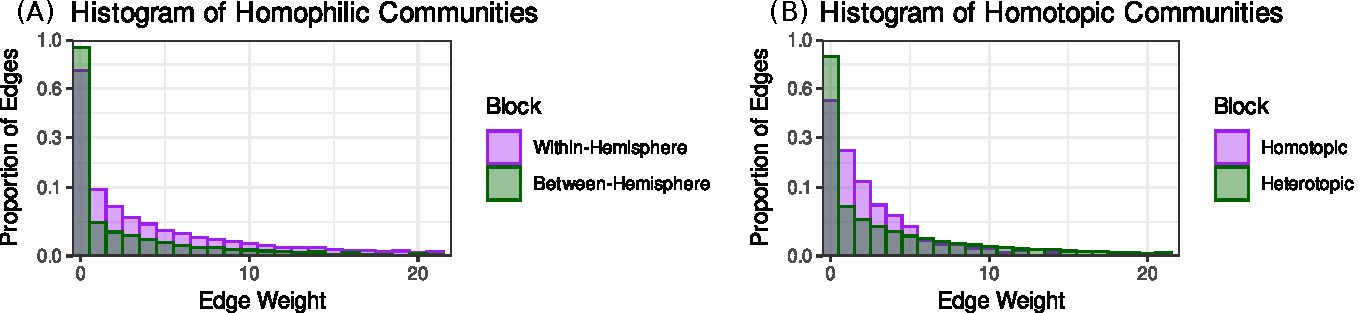
\includegraphics[width=\linewidth]{figures/dros_siem.pdf}
    \caption{\textbf{Goodness of fit of homophilic and homotopic $\siem$ for weighted \textit{Drosophila} mushroom body}. \textbf{(A)} A comparison of the homophilic communities as determined by the hemispheres of incident vertices. The relative heights of the bars are normalized by the square root of the proportion due to the fact that the substantial majority of edges in both communities have a weight of $0$. Within-hemisphere edges appear to have greater connectivity than between-hemisphere edges. Within-hemisphere edges show significantly higher connectivity than between-hemisphere edges (Mann-Whitney Wilcoxon Test, $n=103041$, $p$-value$=0.0$). \textbf{(B)} A comparison of the homotopic edge communities, where homotopic edges are those that are incident a bilateral pair of vertices. Homotopic edges appear to have greater connectivity than heterotopic edges. Homotopic connectivity significantly exceeds heterotopic connectivity (Mann-Whitney Wilcoxon Test, $n=103041$, $p$-value$=0.0$).}
    \label{fig:dros_siem}
\end{figure}

In Figure \ref{fig:siem_os_mri} we explore the appropriateness of the $\siem$ for diffusion connectomes from the HCP Dataset. Figure \ref{fig:siem_os_mri}(A) shows the average diffusion connectome over all participants in the study. Figure \ref{fig:siem_os_mri}(B) shows the distribution of edge-weights within-hemisphere versus between-hemisphere. The diffusion connectomes appear to possess homophily; ie, high within-hemisphere connectivity, with lower between-hemisphere connectivity. To test this observation, we employ the $\texttt{MWW}$ test. All $1059$ diffusion connectomes have significantly higher within-hemisphere connectivity than between-hemisphere connectivity at $\alpha=.05$ after Bonferroni correction \cite{Bonferroni1936-ip}.

\begin{figure}
    \centering
    \includegraphics[width=\linewidth]{figures/hcp_siem.pdf}
    \caption{\textbf{Goodness of fit of homophilic $\siem$ for diffusion connectomes}. \textbf{(A)} The average diffusion connectome over $N=1059$ connectomes with $n=70$ vertices from the HCP dataset shows that diffusion connectomes appear to be homophilic, with higher within-hemisphere connectivity than between-hemisphere connectivity. Hemisphere annotations are provided for regions in the left and right hemispheres. Within-hemisphere edges are edges whose vertices are both located in the same hemisphere of the brain (the on-diagonal blocks). \textbf{(B)} Density estimates for the within-hemisphere and between-hemisphere edges for each of the $N=1059$ connectomes. Homophily is tested per-graph using the Mann-Whitney Wilcoxon Test to detect whether the on-diagonal blocks have higher connectivity than the off-diagonal blocks. All $N=1059$ diffusion connectomes have significantly higher within-hemisphere connectivity than between-hemisphere connectivity after Bonferroni correction at $\alpha=.05$, and the maximum corrected $p$-value is on the order of $10^{-21}$.}
    \label{fig:siem_os_mri}
\end{figure}

\subsection{Identification of Optimal Block Structure}\label{sec:sbm_est_wt}

In Figure \ref{fig:dros_sbm_est}, we investigate the appropriate block structure for the weighted \textit{Drosophila} mushroom body. \ref{fig:dros_sbm_est}(I) shows the distribution of edges associated with each block of $\B$, where the $n=319$ vertices in either the left or right hemisphere are partitioned according to hemisphere. Again, the weighted \textit{Drosophila} mushroom body is directed, so assuming symmetry would not be sensible. We investigate whether the \textit{Drosophila} mushroom body is $\er$, planted partition, symmetric heterogeneous, or asymmetric heterogeneous $\sbm$, using Kruskal-Wallis (KW), Distance Correlation (DCorr), and Analysis of Variance (ANOVA). Each method identifies the planted partition $\sbm$ as the most appropriate block model. This has the interpretation that the best-fit $\sbm$ includes a shared distribution for the on-diagonal (Left,Left) and (Right,Right) blocks, and a different shared distribution for the off-diagonal (Left,Right) and (Right,Left) blocks. An important considerations is that while the best-fit $\sbm$ is symmetric, the graph itself is directed. This has the implication that while the best-fit $\sbm$ would posit that edges in the (Left,Right) and (Right,Left) blocks have the same distribution, realizations of the (Left,Right) and (Right,Left) block will not necessarily be identical.

\begin{figure}
    \centering
    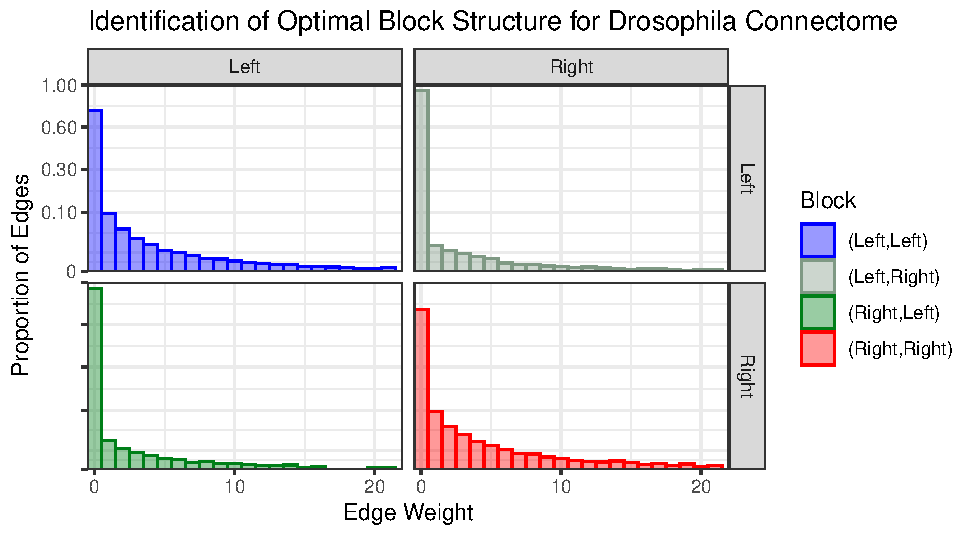
\includegraphics[width=.8\linewidth]{figures/dros_sbm_est.pdf}
    \caption{\textbf{Identifying the appropriate block structure of the \textit{Drosophila} mushroom body}. We investigate the appropriate block structure in the \textit{Drosophila}  mushroom body, with $n=319$ vertices in the left or right hemisphere. Each block corresponds to the proportion of edges with the listed edge weight. As in Figure \ref{fig:dros_siem}, the proportion of edges are shown on a scale in which bar height corresponds to the square root of the proportion, due to the presence of a large number of zero-weight edges. We investigate whether the $\sbm$ is $\er$, planted partition, symmetric heterogeneous, or asymmetric heterogeneous $\sbm$, using Kruskal-Wallis (KW), Distance Correlation (DCorr), and Analysis of Variance (ANOVA) for model selection. All approaches identify planted partition $\sbm$ as the best-fit block structure.}
    \label{fig:dros_sbm_est}
\end{figure}

In Figure \ref{fig:nested_sbm_ts_mri}, we investigate the appropriate block structure for diffusion connectomes, analogous to the single graph investigations using the \textit{Drosophila} mushroom body in Figure \ref{fig:dros_sbm_est}. Panel \textbf{(A)} demonstrates the distribution of edges associated with each block of $\B$. Panel \textbf{(B)} shows the fraction of diffusion connectomes that accept each of the candidate hypotheses, using $3$ different approaches for weighted graph model selection: Kruskal-Wallace  \cite{Kruskal1952-kj}, Distance Correlation (Dcorr) \cite{Szekely2007-mm}, and Ananysis of Variance (ANOVA) \cite{Fisher1925-xm,Scheffe1999-pi}. Diffusion connectomes tend to display planted partition structure across all model selection approaches.

\begin{figure}
    \centering
    \includegraphics[width=\linewidth]{figures/hcp_block_est.pdf}
    \caption{\textbf{Identification of appropriate block structure in diffusion connectomes}. We investigate the appropriate block structure in the diffusion connectomes from the HCP Dataset, with $n=70$ vertices, and $N=1059$ graphs. \textbf{(A)} the empirical distribution of edges for each of the $4$ blocks of edges for each between and within-hemisphere pair for the left and right hemispheres respectively. As the diffision connectomes are inherently symmetric, the off-diagonal blocks are inherently symmetric. The hypothesized models are that the graph is $\er$, planted partition $\sbm$ (Plant Part.), or the symmetric heterogeneous $\sbm$ (Sym. Het.). \textbf{(B)} The number of connectomes from the dataset for which the specified candidate model is selected. All methods for selection of optimal block structure identify diffusion connectomes as planted partition $\sbm$, which has the interpretation that the optimal structure is to assume that the on-diagonal left and right blocks share a common distribution that differs from the off-diagonal contralateral blocks. This conclusion holds across all diffusion connectomes within the dataset.}
    \label{fig:nested_sbm_ts_mri}
\end{figure}



\section{Multiple Graph Applications}\label{sec:multi_app_appendix}

\subsection{Testing for Significant Edges in Weighted Networks} \label{sec:exp2}
We consider two populations of networks generated from a 2 block $\sbm$, except edges are now sampled from truncated normal distribution to emulate correlation matrices. All networks have $n=20$ vertices and $\vec{\pi} = \bracks*{0.25, 0.75}$. The block edge distribution matrices for each population is given by
\begin{align*}
    \B^{(1)} &= 
    \begin{bmatrix}
        \tnorm(0, 0.25, -1, 1)   & \tnorm(0, 0.25, -1, 1) \\
        \tnorm(0, 0.25, -1, 1)   & \tnorm(0, 0.25, -1, 1) 
    \end{bmatrix} \\
    \B^{(2)} &= 
    \begin{bmatrix}
        \tnorm(0 + \delta, 0.25 + \phi, -1, 1)   & \tnorm(0, 0.25, -1, 1) \\
        \tnorm(0, 0.25, -1, 1)   & \tnorm(0, 0.25, -1, 1) 
    \end{bmatrix}
\end{align*}
where $\tnorm(\mu, \sigma^2, a, b)$ denotes a truncated normal distribution with mean $\mu$ and variance $\sigma^2$ such that all values are in $[a, b]$. Total of $m$ networks are sampled ($m/2$ networks per population). One population has the same edge weight distribution for all edges, and the second population's first block edges has either a different mean, $\delta$, or variance, $0.25 + \phi$.
For each edge, test statistics are computed with three different tests: 1) t-test, 2) Mann-Whitney (MW) U test, which is a non-parametric test of medians, and 3) two-sample Kolomogrov-Smirnov (KS) test, which is test of two distributions. Similar to experiment 1, the test statistics are sorted to find the ten most significant edges, and the performance is evaluated with recall.

Figure \ref{fig:exp2} shows the results by varying the sample size, mean, and variance. Figure \ref{fig:exp2} top row shows that all three tests can identify edges that are different in means, and that no particular test is superior than another. 
%Even at low sample sizes ($m=100$), all three tests can perfectly identify significant edges At effect size as low as $\delta = 0.3$ with sample size $m=1000$.
Figure \ref{fig:exp2} bottom row shows that only KS test can detect changes in variance when the means are kept the same. This is because t-test and MW test ultimately test for differences in centrality (e.g. mean or median), where as KS tests for any differences between a pair of observed distributions. 
% but large samples size ($m=1000$) and large effect size ($\phi\geq 2.5$) are required for high recall. 

\begin{figure}
    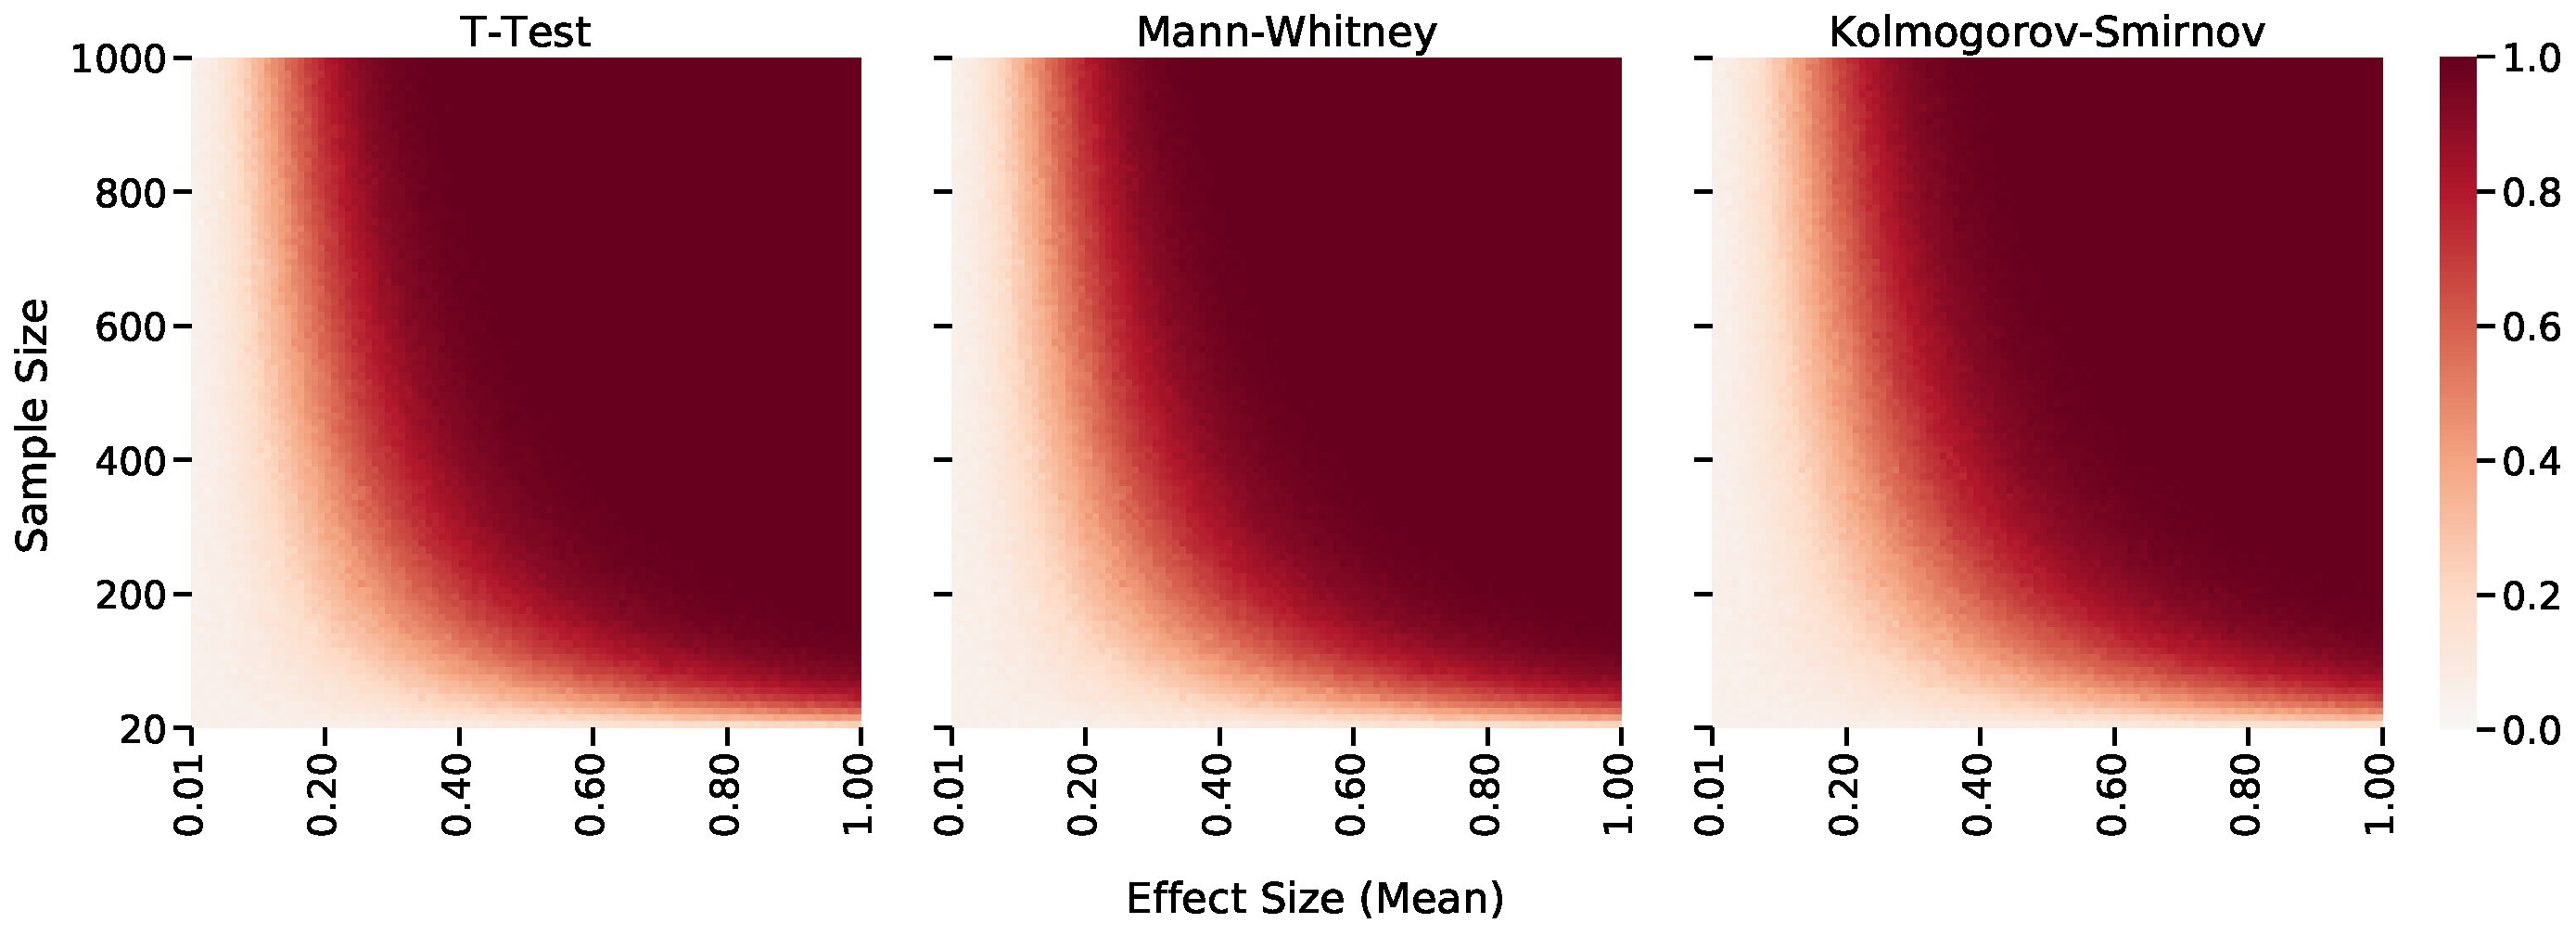
\includegraphics[width=.9\textwidth]{figures/exp2_change_mean}
    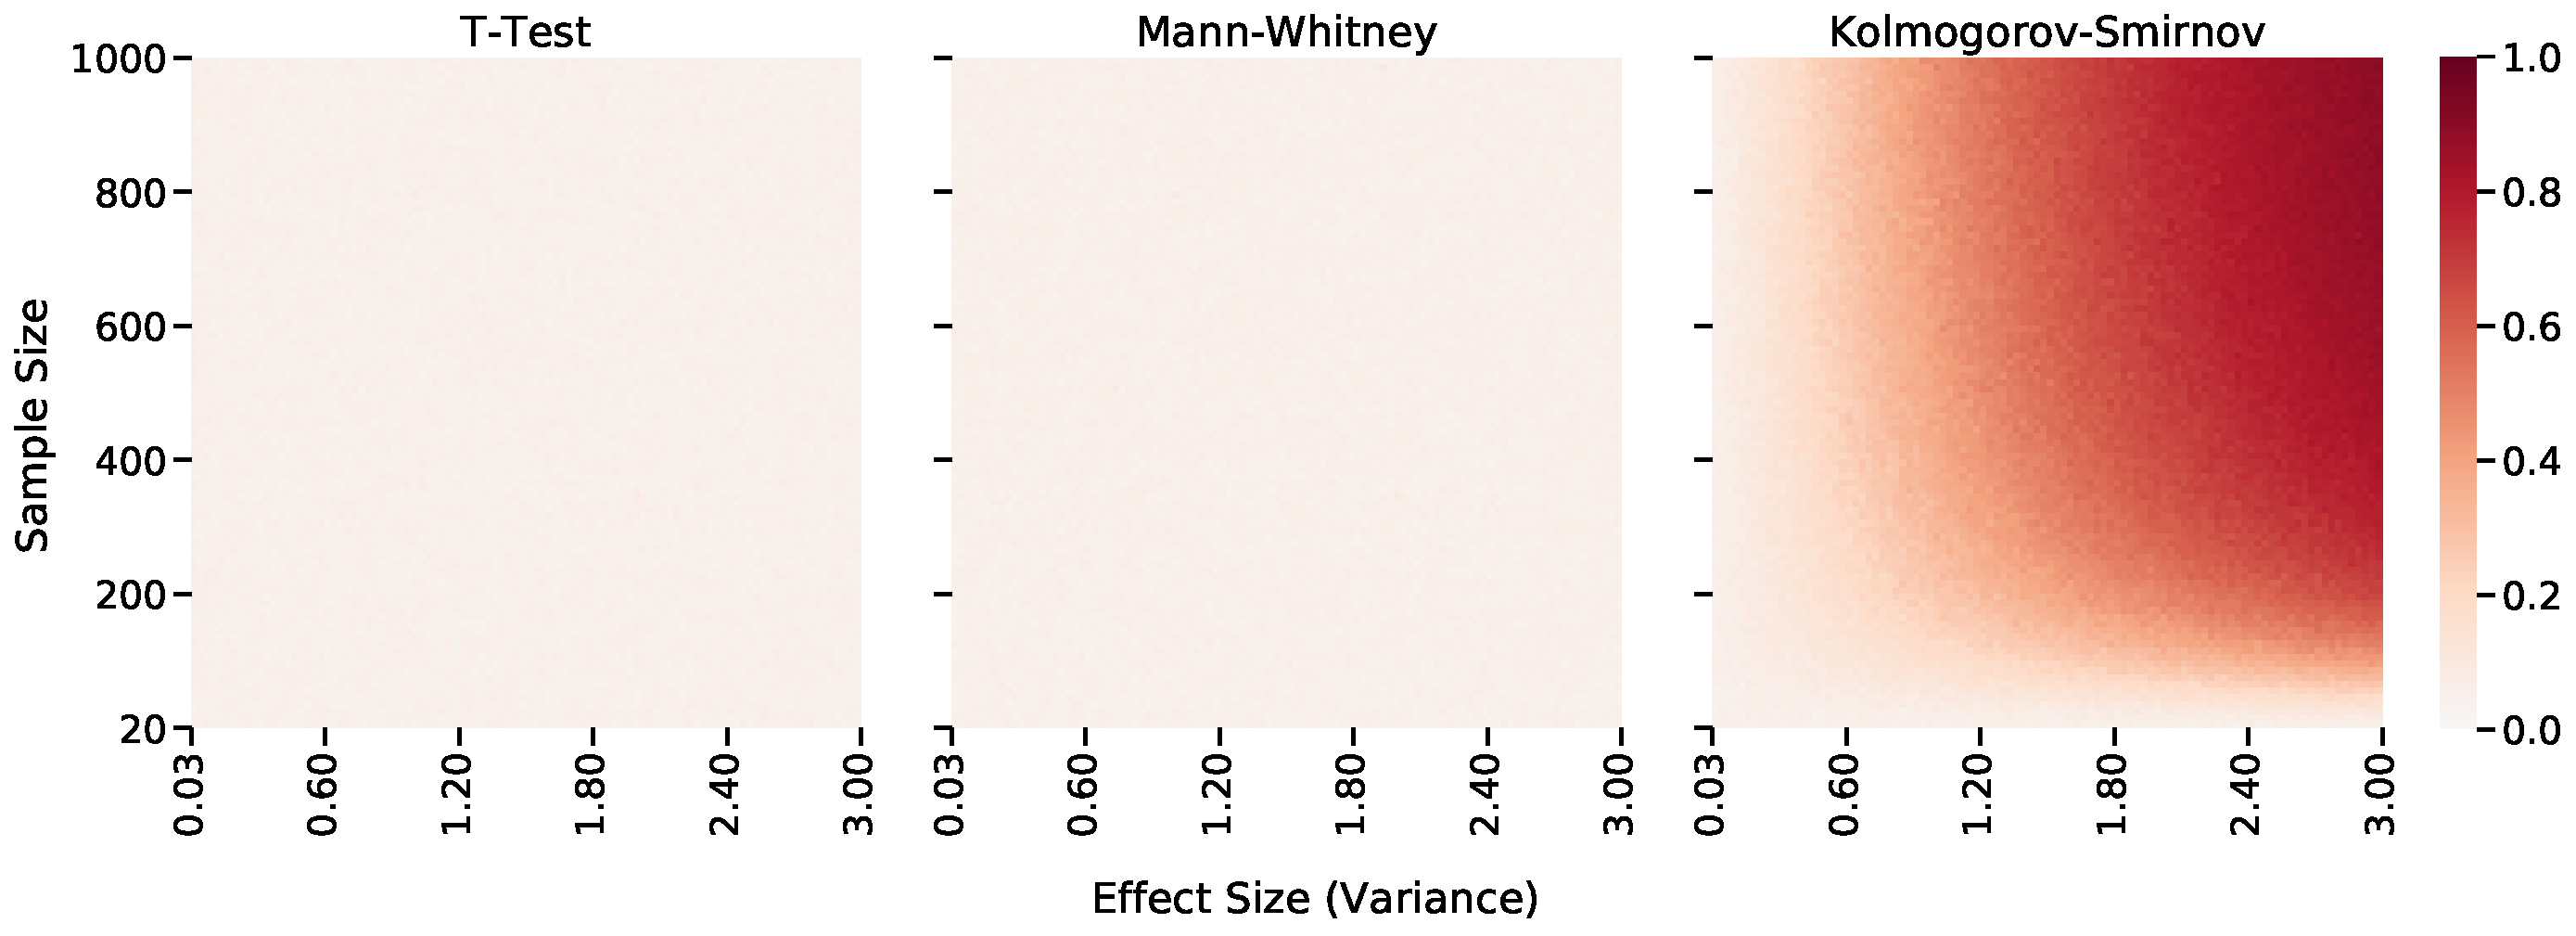
\includegraphics[width=.9\textwidth]{figures/exp2_change_vars}
    \caption{
    \textbf{Performance of finding significant edges that have different weight distributions.}
    Recall@10 for each edge when comparing two populations of weighted networks using t-test, Mann-Whitney, and Kolmogorov-Smirnov tests. The color bar represents recall averaged over 100 trials. 
    \textit{(Top row)} Results for varying the mean $\delta$ and sample size wile keeping the variance is same ($\phi = 0$). All three tests perform equally, and can detect significant edges when edge distributions differ in means.
    \textit{(Bottom row)} Results for varying the variance $\phi$ and sample size wile keeping the mean same ($\delta = 0$). T-test and Mann-Whitney test cannot detect changes in variance regardless of the sample and effect size. KS test is the only test that can detect changes in variance.}
    \label{fig:exp2}
\end{figure}

Functional connectivity in human brains was analyzed using functional connectomes estimated using fMRI data from the HCP dataset. In functional connectomes, the edges represent correlations of changes in blood flow between a pair of ROIs, which is a proxy for correlations of brain activity. For each edge, the class-conditional mean and the variance of truncated normal distribution are computed for males ($m=330$) and females ($m=407$). Networks are then simulated as above using the 2-block weighted $\sbm$, but the parameters for first block, $\B_{11}$, is substituted with class-conditional means and variances. The performance is measured with recall@10, denoted empirical trustworthiness in Figure \ref{fig:exp2_hcp}, is measured using KS test. Again, the empirical trustworthiness shows how one can trust that the edge is truly different. There are 70 vertices with 2380 total edges, but only 256 edges have trustworthiness $\geq 0.9$.

\begin{figure}
    \centering
    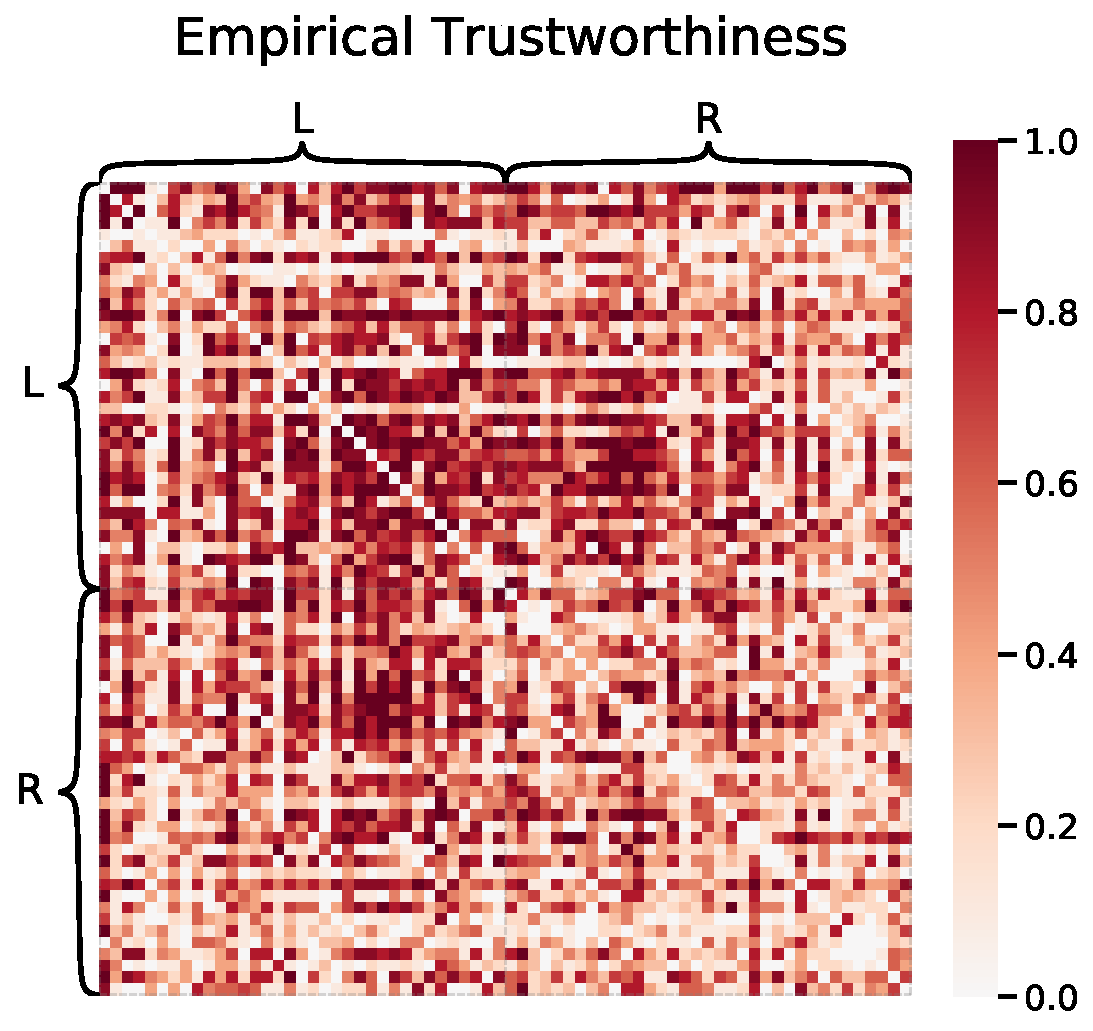
\includegraphics[width=0.45\textwidth]{figures/exp2_empirical_trustworthiness}
    \caption{
    Functional connectomes are derived from the HCP data. Vertices are defined by Desikan parcellation into 70 ROIs, and are organized by hemisphere, denoted left hemisphere (L) and right hemisphere (R). Edge weights are correlations represent correlation of brain activity between a pair of ROIs. 
    For each edge, the class-conditional means and the variances for females ($m=407$) and males ($m=330$) are computed, which are used to simulate weighted 2-block $\sbm$. Recall@10, denoted empirical trustworthiness, is measured from test statistics using KS test. Out of the 2380 total edges, only 256 edges have trustworthiness $\geq 0.9$. 
    }
    \label{fig:exp2_hcp}
\end{figure}


% \begin{summary}[SUMMARY POINTS]
% When comparing two populations of weighted networks for significantly different edges, t-test can detect changes in means, but cannot detect changes in variances. Distribution free tests, such as Kologrov-Smirnov test can detect changes in both means and variances.
% \end{summary}

\subsection{Testing for Significant Edges Using Communities in Binary Networks} \label{sec:exp3}
In previous section \ref{sec:exp1}, the community structure was ignored even though the generative process produced two communities. In the following experiment, the community assignments are used to test whether all edges within a community or across communities are significantly different. Formally, the following hypothesis test is considered: 
\begin{align*}
    H_0:~ \PP[\B_{ij}|Y=0] = \PP[\B_{ij}|Y=1]\\
    H_A:~  \PP[\B_{ij}|Y=0]\neq \PP[\B_{ij}|Y=1]
\end{align*}
where $\PP[\B_{ij}|Y=y]$ denotes class-conditional distribution of edges that belong to community $i$ and $j$, and $i, j\in [K]$ where $K$ denotes the number of communities. When $i =j$, the edges are incident to vertices that belong to the same community. When $i\neq j$, the edges are incident to vertices that do not belong in the same community. In this setting, a total of $\frac{(K)(K+1)}{2}$ null hypothesis are tested.  

We consider two populations of networks with the connectivity probability matrices as below, 
\begin{align*}
\B^{(1)} = 
    \begin{bmatrix}
    p & p \\ p & p
    \end{bmatrix},~
\B^{(2)} = 
    \begin{bmatrix}
    p+\delta & p \\ p & p
    \end{bmatrix}
\end{align*}
with $n=50$ vertices, and membership vector, $\vec{\pi} = \bracks*{0.5, 0.5}$. Total of $m$ networks are sampled ($m/2$ networks per population). Since $K=2$, community assignment results in three sets of edges, two within communities and one across communities. The t-test statistic was computed for each set of edges, and significant edges are identified by the hypothesis test that resulted in largest test-statistic. The performance is measured by precision, which measures false positive rate, and recall, which measures true positive rate.

Figure \ref{fig:exp3} shows the results of using t-test as the effect size is changed using known and estimated community assignments. When the community assignment is known \textit{a priori}, significant edges can be perfectly detected with no false positives at low sample sizes ($m=10$) and effect size ($\delta \geq 0.05$). However, estimating community assignments results in large number of false positives edges as shown in precision plots for both $\jrdpg$ and $\cosie$ models since recovery of community assignments is correlated with magnitude of the effect size. When effect size is small, communities cannot be reliably recovered for both $\jrdpg$ and $\cosie$ models, which results in false positive tests. As effect size increases, community recovery improves and the number of false positive edges decrease at effect size ($\delta \geq 0.2$). 

\begin{figure}
    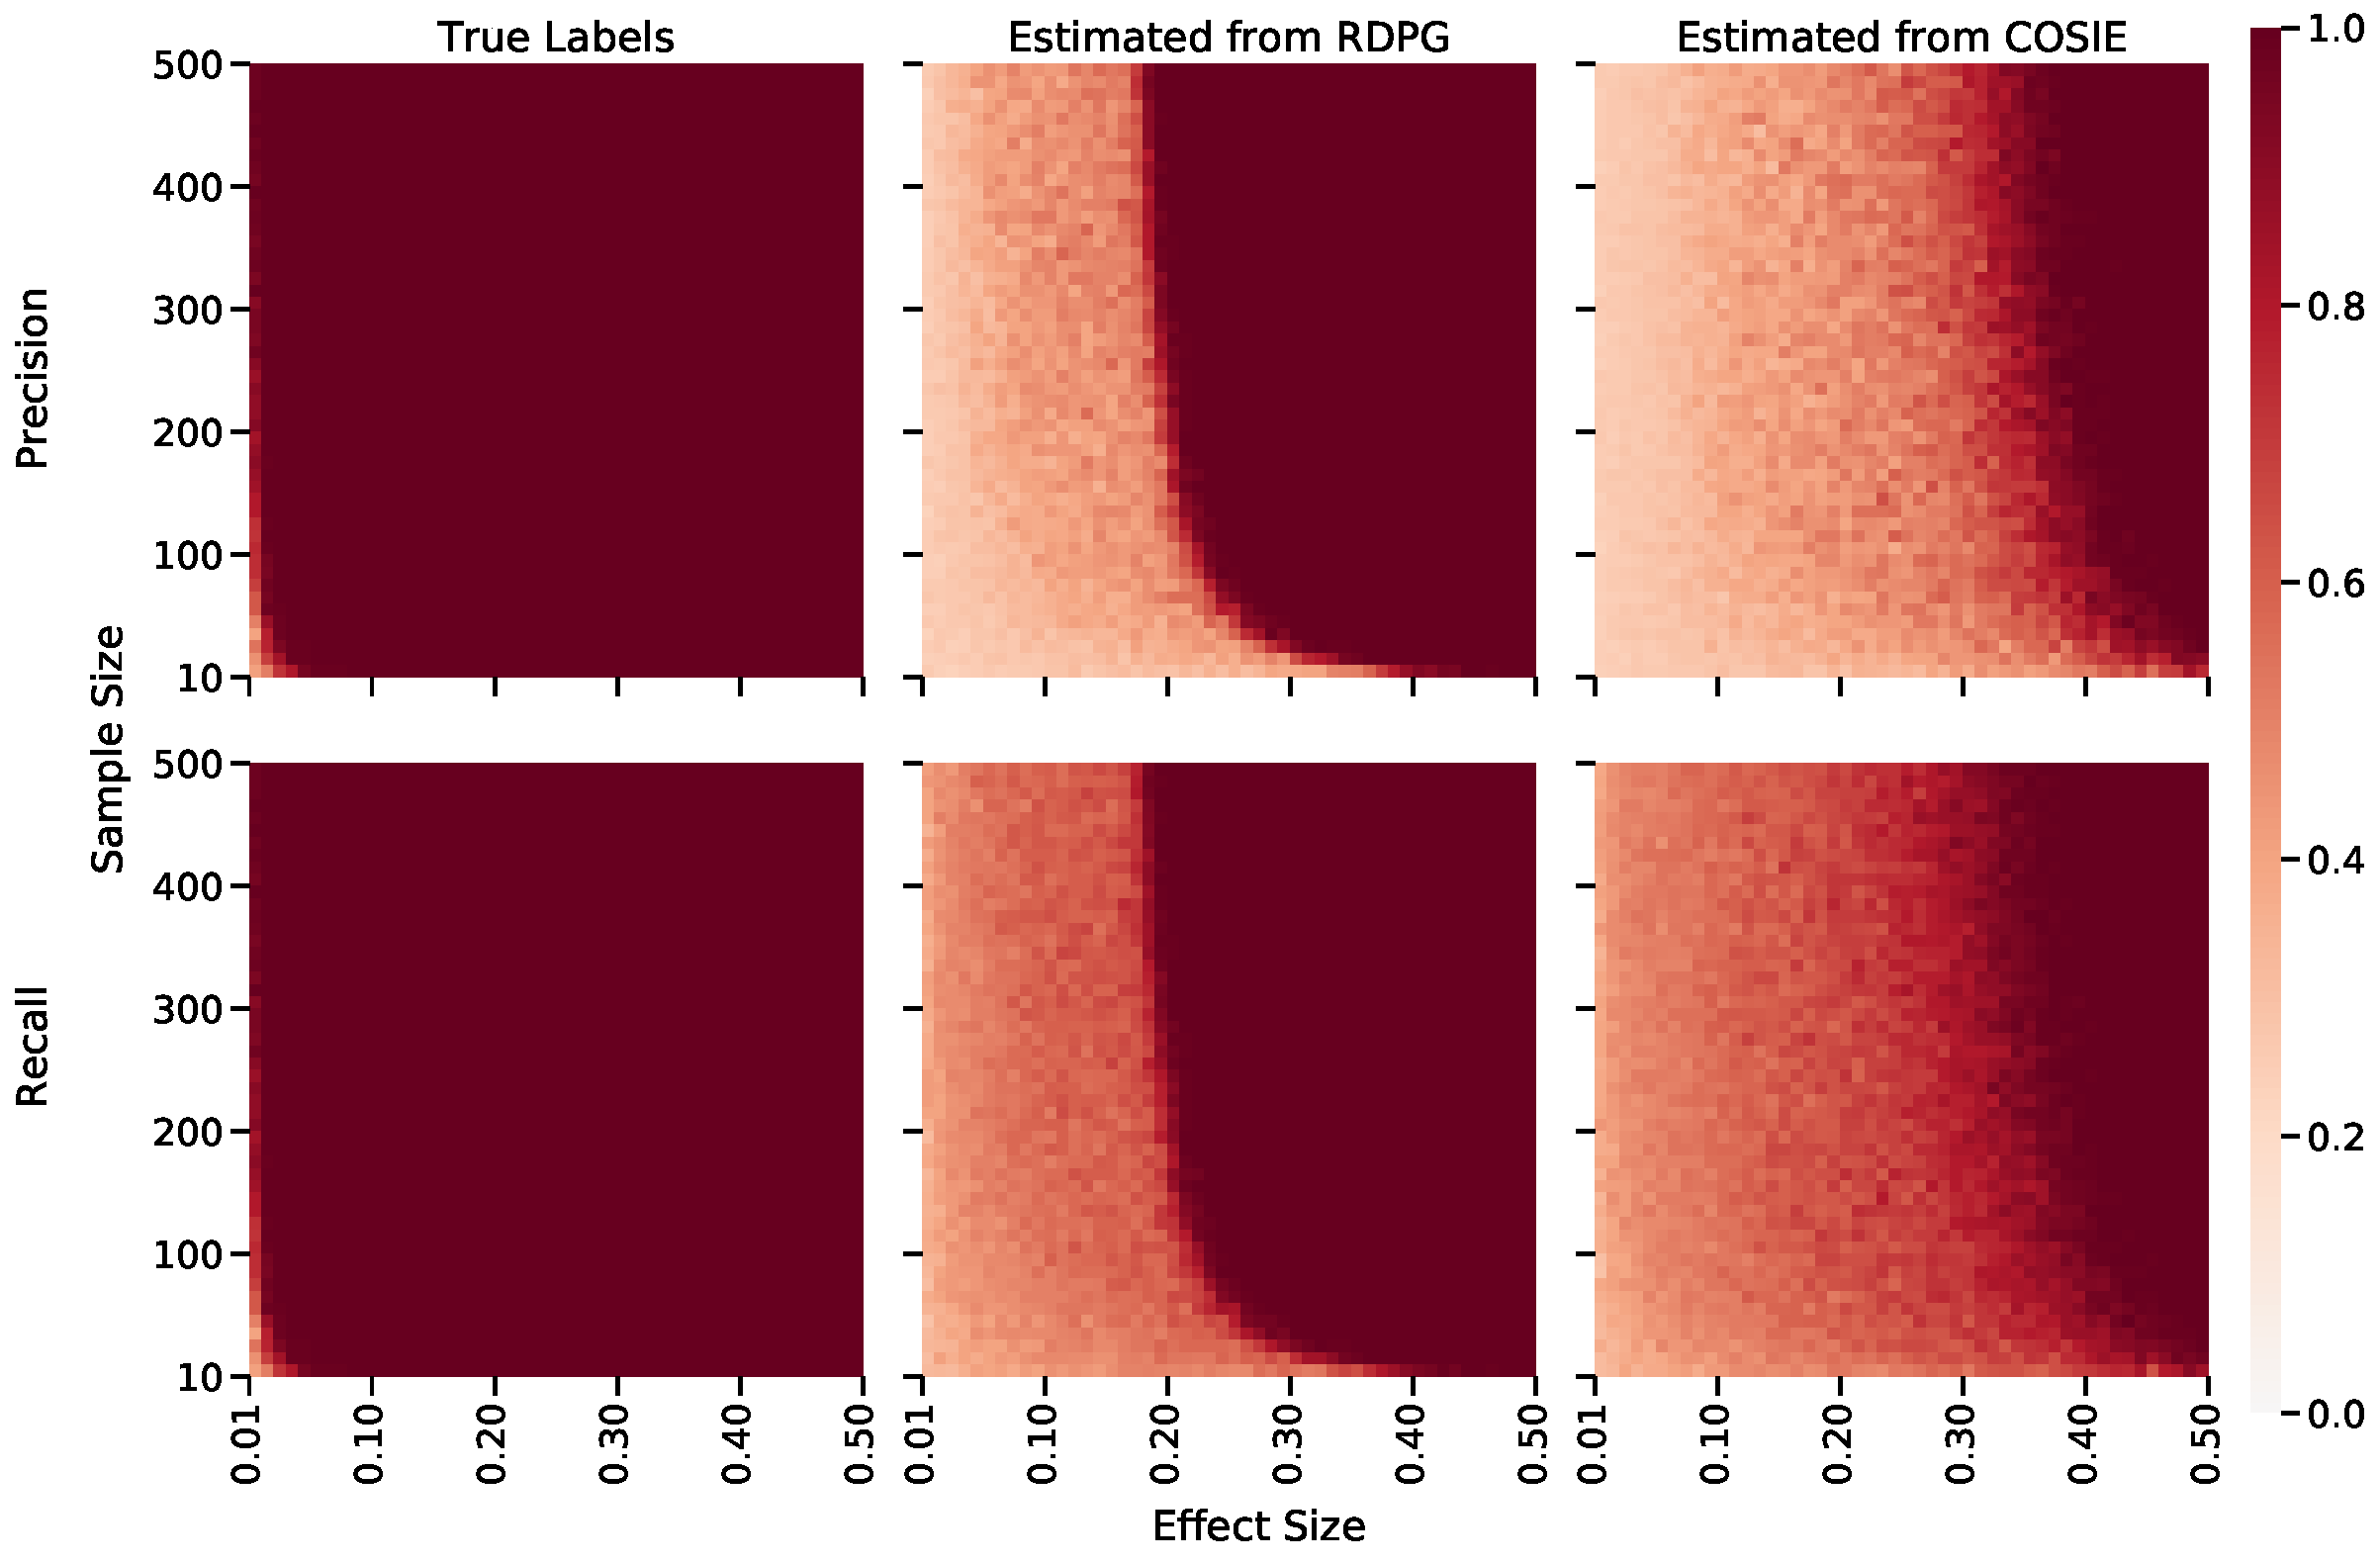
\includegraphics[width=.9\textwidth]{figures/exp3_final}
    \caption{
    \textbf{Performance of finding significant edges using either known or estimated community structure.}
    Precision \textit{(top row)} and recall \textit{(bottom row)} for
    significant edges using t-test on sets of edges from within community or across communities averaged over 50 trials.
    \textit{(Left column)} shows the precision and recall when using true community assignments. At low sample sizes ($m =10$) and low effect size ($\delta \geq 0.05$), community wise testing results in perfect precision and recall.
    \textit{(Middle column)} shows the results for using community assignments estimated under the $\jrdpg$ model. 
    \textit{(Right column)} shows the results for using community assignments estimated under the  $\cosie$ model. 
    Since recovery of community assignment is related to the effect size, spectral clustering results in misclassified vertices. As a result, precision is low at effect sizes $\leq 0.2$. As effect size increases, the communities become more identifiable, and results in increased precision for $\jrdpg$ and $\cosie$ models. However, COSIE model requires larger effect size to reach precision $\geq 0.95$.
    }
    \label{fig:exp3}
\end{figure}


% The same analysis was performed using binarized structural connectomes from HCP dataset where the connectivity within and across communities are tested between females ($m=407$) and males ($m=407$). Using known hemispheric labels of the vertices, the class-conditional block probabilities are computed and used to simulate 2-block SBMs, and the precision and recall was measured for each hypothesis test. Table \ref{tab:exp3_hcp} shows that in the suggesting that there are differences in the connectivity with and across hemispheres are significantly different in males and females. 

% \begin{table}
%     \caption{Empirical trustworthiness computed using structural connectome from HCP dataset.}
%     \centering
%     \begin{tabular}{c|c|c}
%         \toprule
%         Hypothesis Test &  Empirical Precision & Empirical Recall\\
%         \midrule
%         Right vs Right  &   1   &   1\\
%         Left vs Left    &   1   &   1\\
%         Left vs Right   &   1   &   1\\
%         \bottomrule
%     \end{tabular}
%     \label{tab:exp3_hcp}
% \end{table}

% Show the magnitudes of the test statistics 

% \begin{summary}[SUMMARY POINTS]
% Using community assignments can improve detection of significant edges. When community assignment is know beforehand, community-wise testing can detect significant edges at low sample and effect sizes. 
% When community assignment is not know beforehand, it can be estimated using statistical models. However, community assignment cannot always be trusted, and consequently any subsequent inference, since its performance depends on effect size.
% \end{summary}



\subsection{Testing for Significant Edges Using Communities in Weighted Networks} \label{sec:exp4}

We consider weighted 2-block $\sbm$ similar to that of Section \ref{sec:exp2}, but with $n=50$ vertices, membership vector, $\vec{\pi} = \bracks*{0.5, 0.5}$, and block edge distribution is as below: 
\begin{align*}
    \B^{(1)} &= 
    \begin{bmatrix}
        \tnorm(0, 0.25, -1, 1)   & \tnorm(0, 0.25, -1, 1) \\
        \tnorm(0, 0.25, -1, 1)   & \tnorm(0, 0.25, -1, 1) 
    \end{bmatrix} \\
    \B^{(2)} &= 
    \begin{bmatrix}
        \tnorm(0 + \delta, 0.25 + \phi, -1, 1)   & \tnorm(0, 0.25, -1, 1) \\
        \tnorm(0, 0.25, -1, 1)   & \tnorm(0, 0.25, -1, 1) 
    \end{bmatrix}
\end{align*}
We proceed with the same experiment as that of Section \ref{sec:exp3}, while changing the means ($\delta$) or the variances ($\phi$). The community assignment is estimated using $\omni$ under $\jrdpg$ model and $\mase$ under $\cosie$ model.
The KS test statistic was computed for each set of edges, and significant edges are identified by the hypothesis test that resulted in largest test-statistic.
The performance is measured with precision and recall. 

Figure \ref{fig:exp4_means} shows the results when varying the mean ($\delta$) and Figure \ref{fig:exp4_vars} shows the results when varying the variance ($\phi$). When the community assignment is known \textit{a priori}, significant edges can be perfectly detected with no false positives at low sample sizes ($m=10$) and effect size ($\delta \geq 0.1$, $\phi \geq 0.12$). When means are changed, communities can be perfectly recovered under $\jrdpg$ model, but communities cannot be reliably recovered under $\cosie$ model. When the edge distributions are different by variance, recovering communities is impossible regardless of the statistical model. This suggest that both $\jrdpg$ and $\cosie$ models are not appropriate when studying differences in variances. 

\begin{figure}
    \centering
    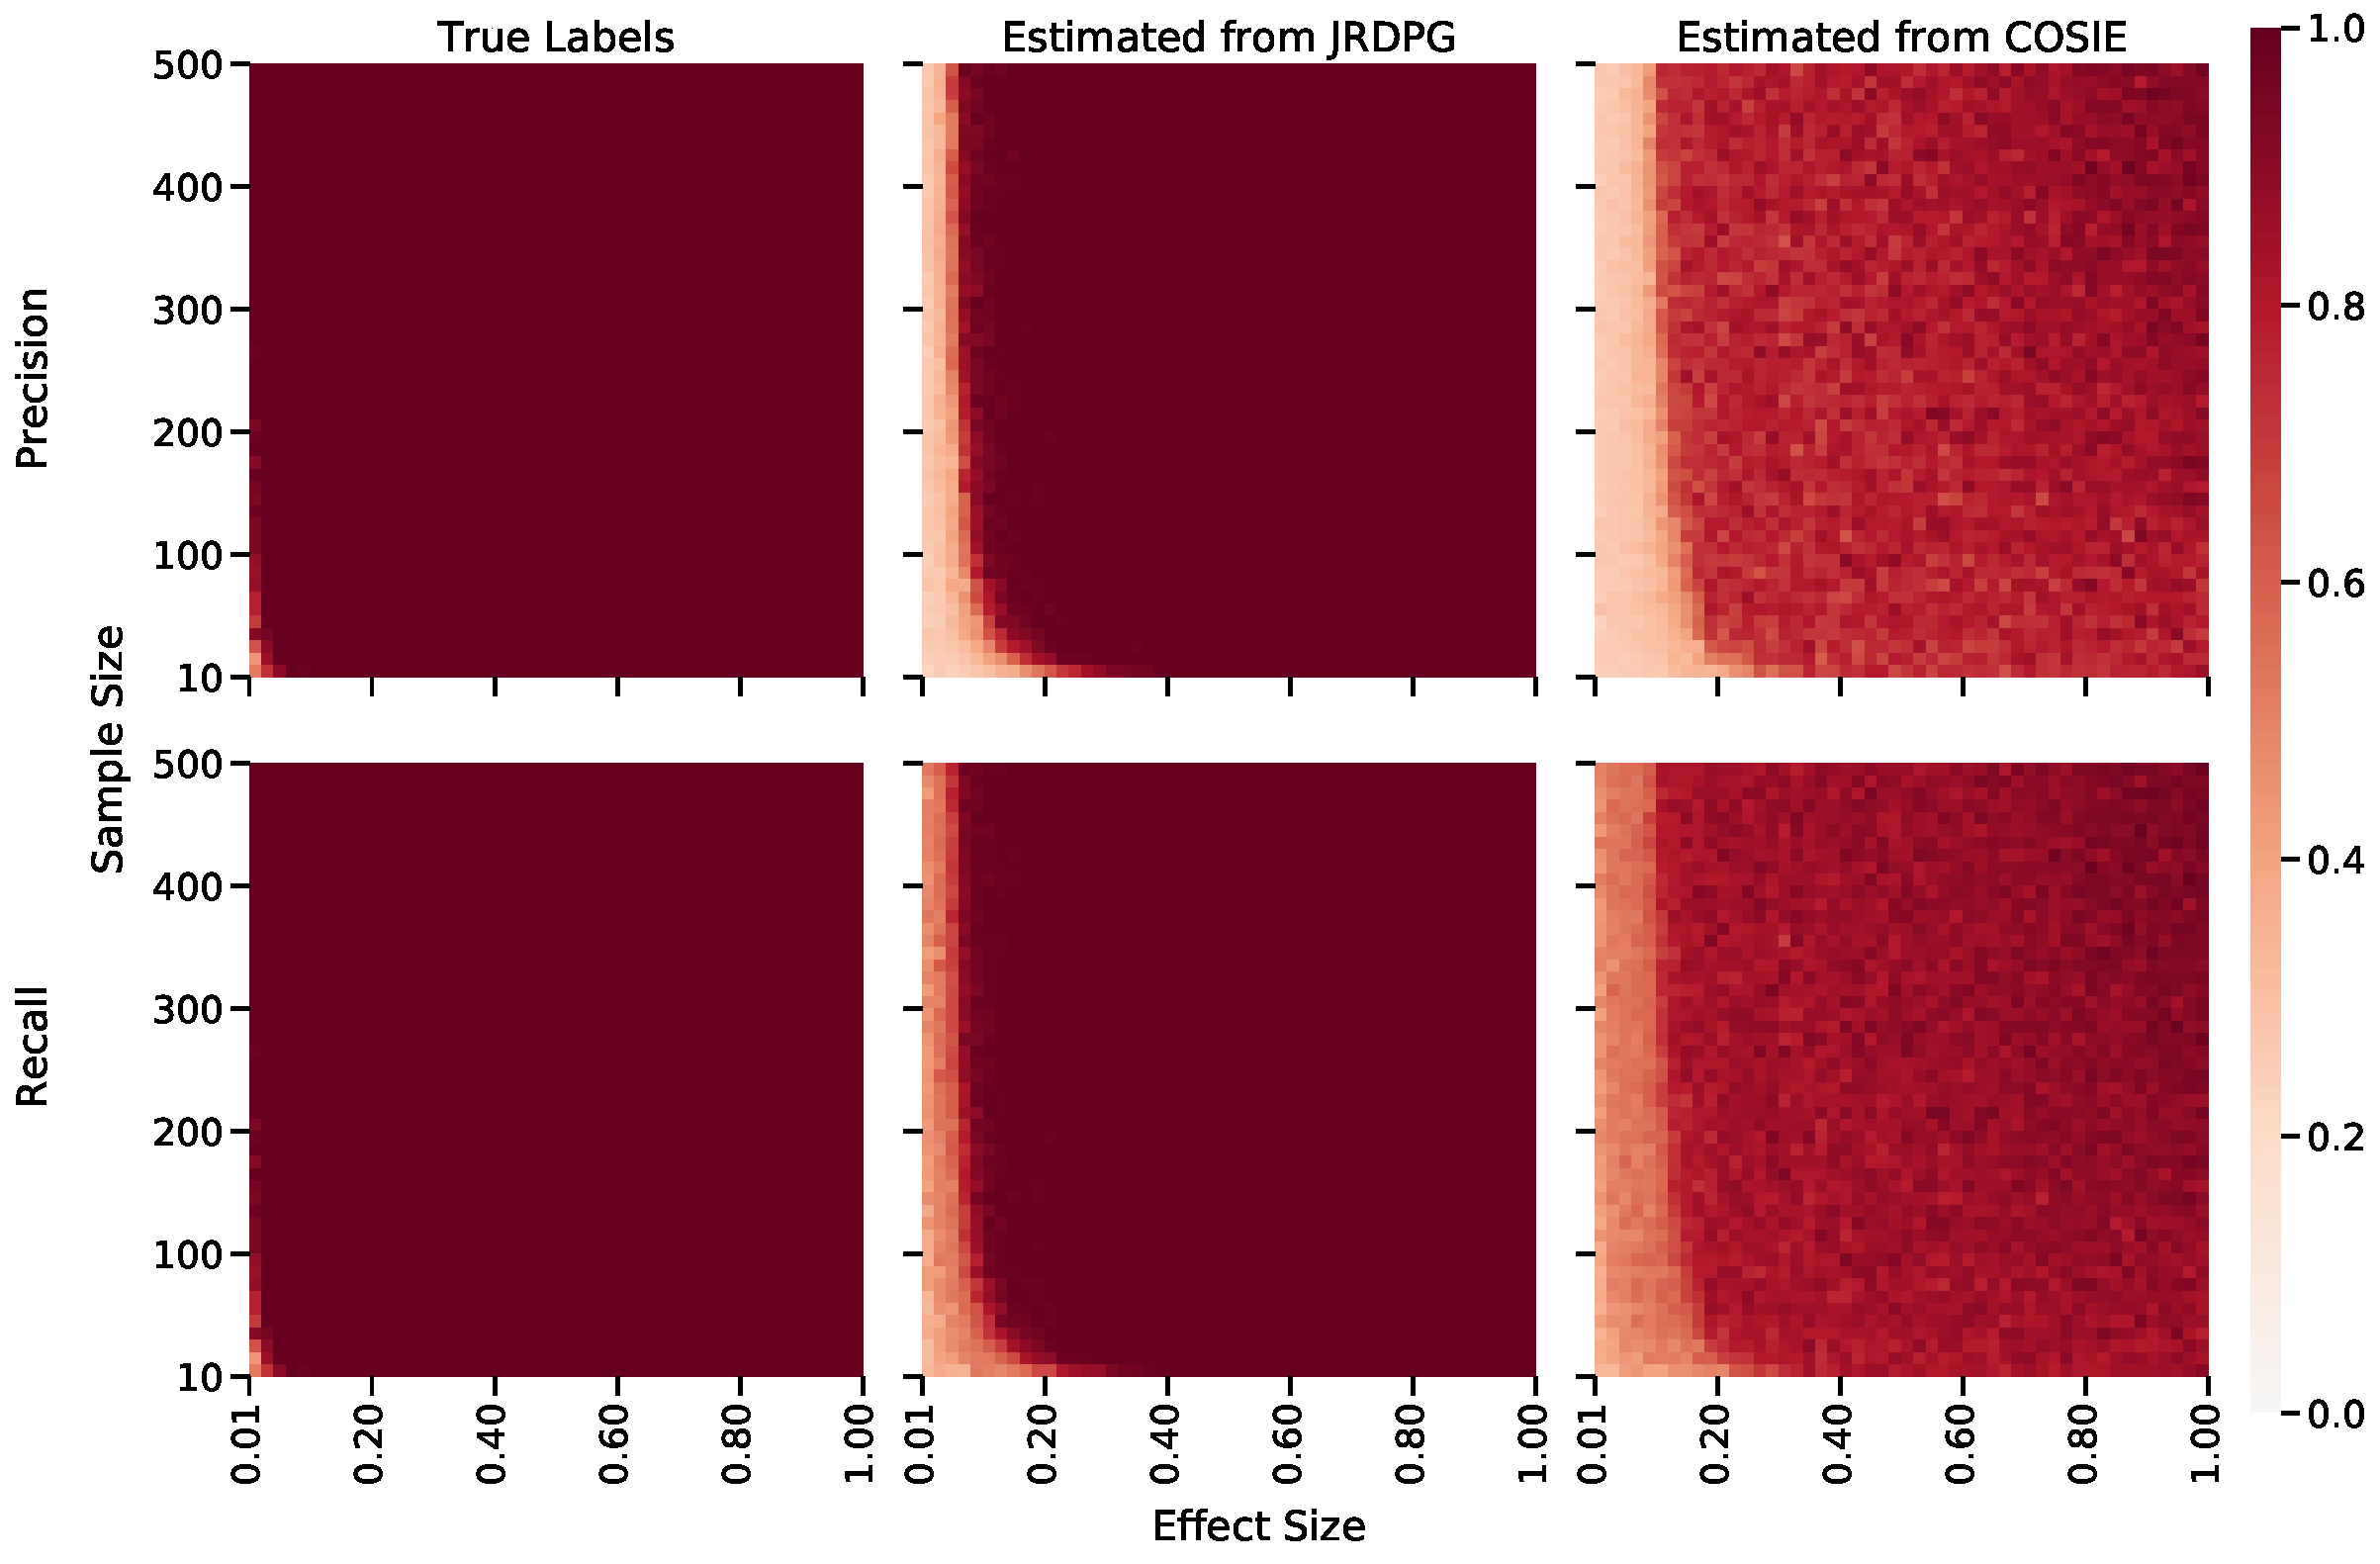
\includegraphics[width=.9\textwidth]{figures/exp4_means_final.pdf}
    \caption{Precision \textit{(top row)} and recall \textit{(bottom row)} for significant edges using $\ks$ test averaged over 50 trials. Effect size (x-axis) is the difference in means of the truncated normal distribution for $\B_{1, 1}$.
    \textit{(Left column)} shows the precision and recall when using known community assignments. At low sample sizes ($m =10$) and low effect size ($\delta \geq 0.1$), community wise testing results in perfect precision and recall.
    \textit{(Middle column)} shows the results for using community assignments estimated under the $\jrdpg$ model. Even at low effect size ($\delta \geq 0.15$), communities can be perfectly recovered. All significant edges can be detected without false positives. 
    \textit{(Right column)} shows the results for using community assignments estimated under the $\cosie$ model. Under this model, communities cannot be perfectly recovered, resulting in false positive edges and false negative edges.}
    \label{fig:exp4_means}
\end{figure}

\begin{figure}
    \centering
    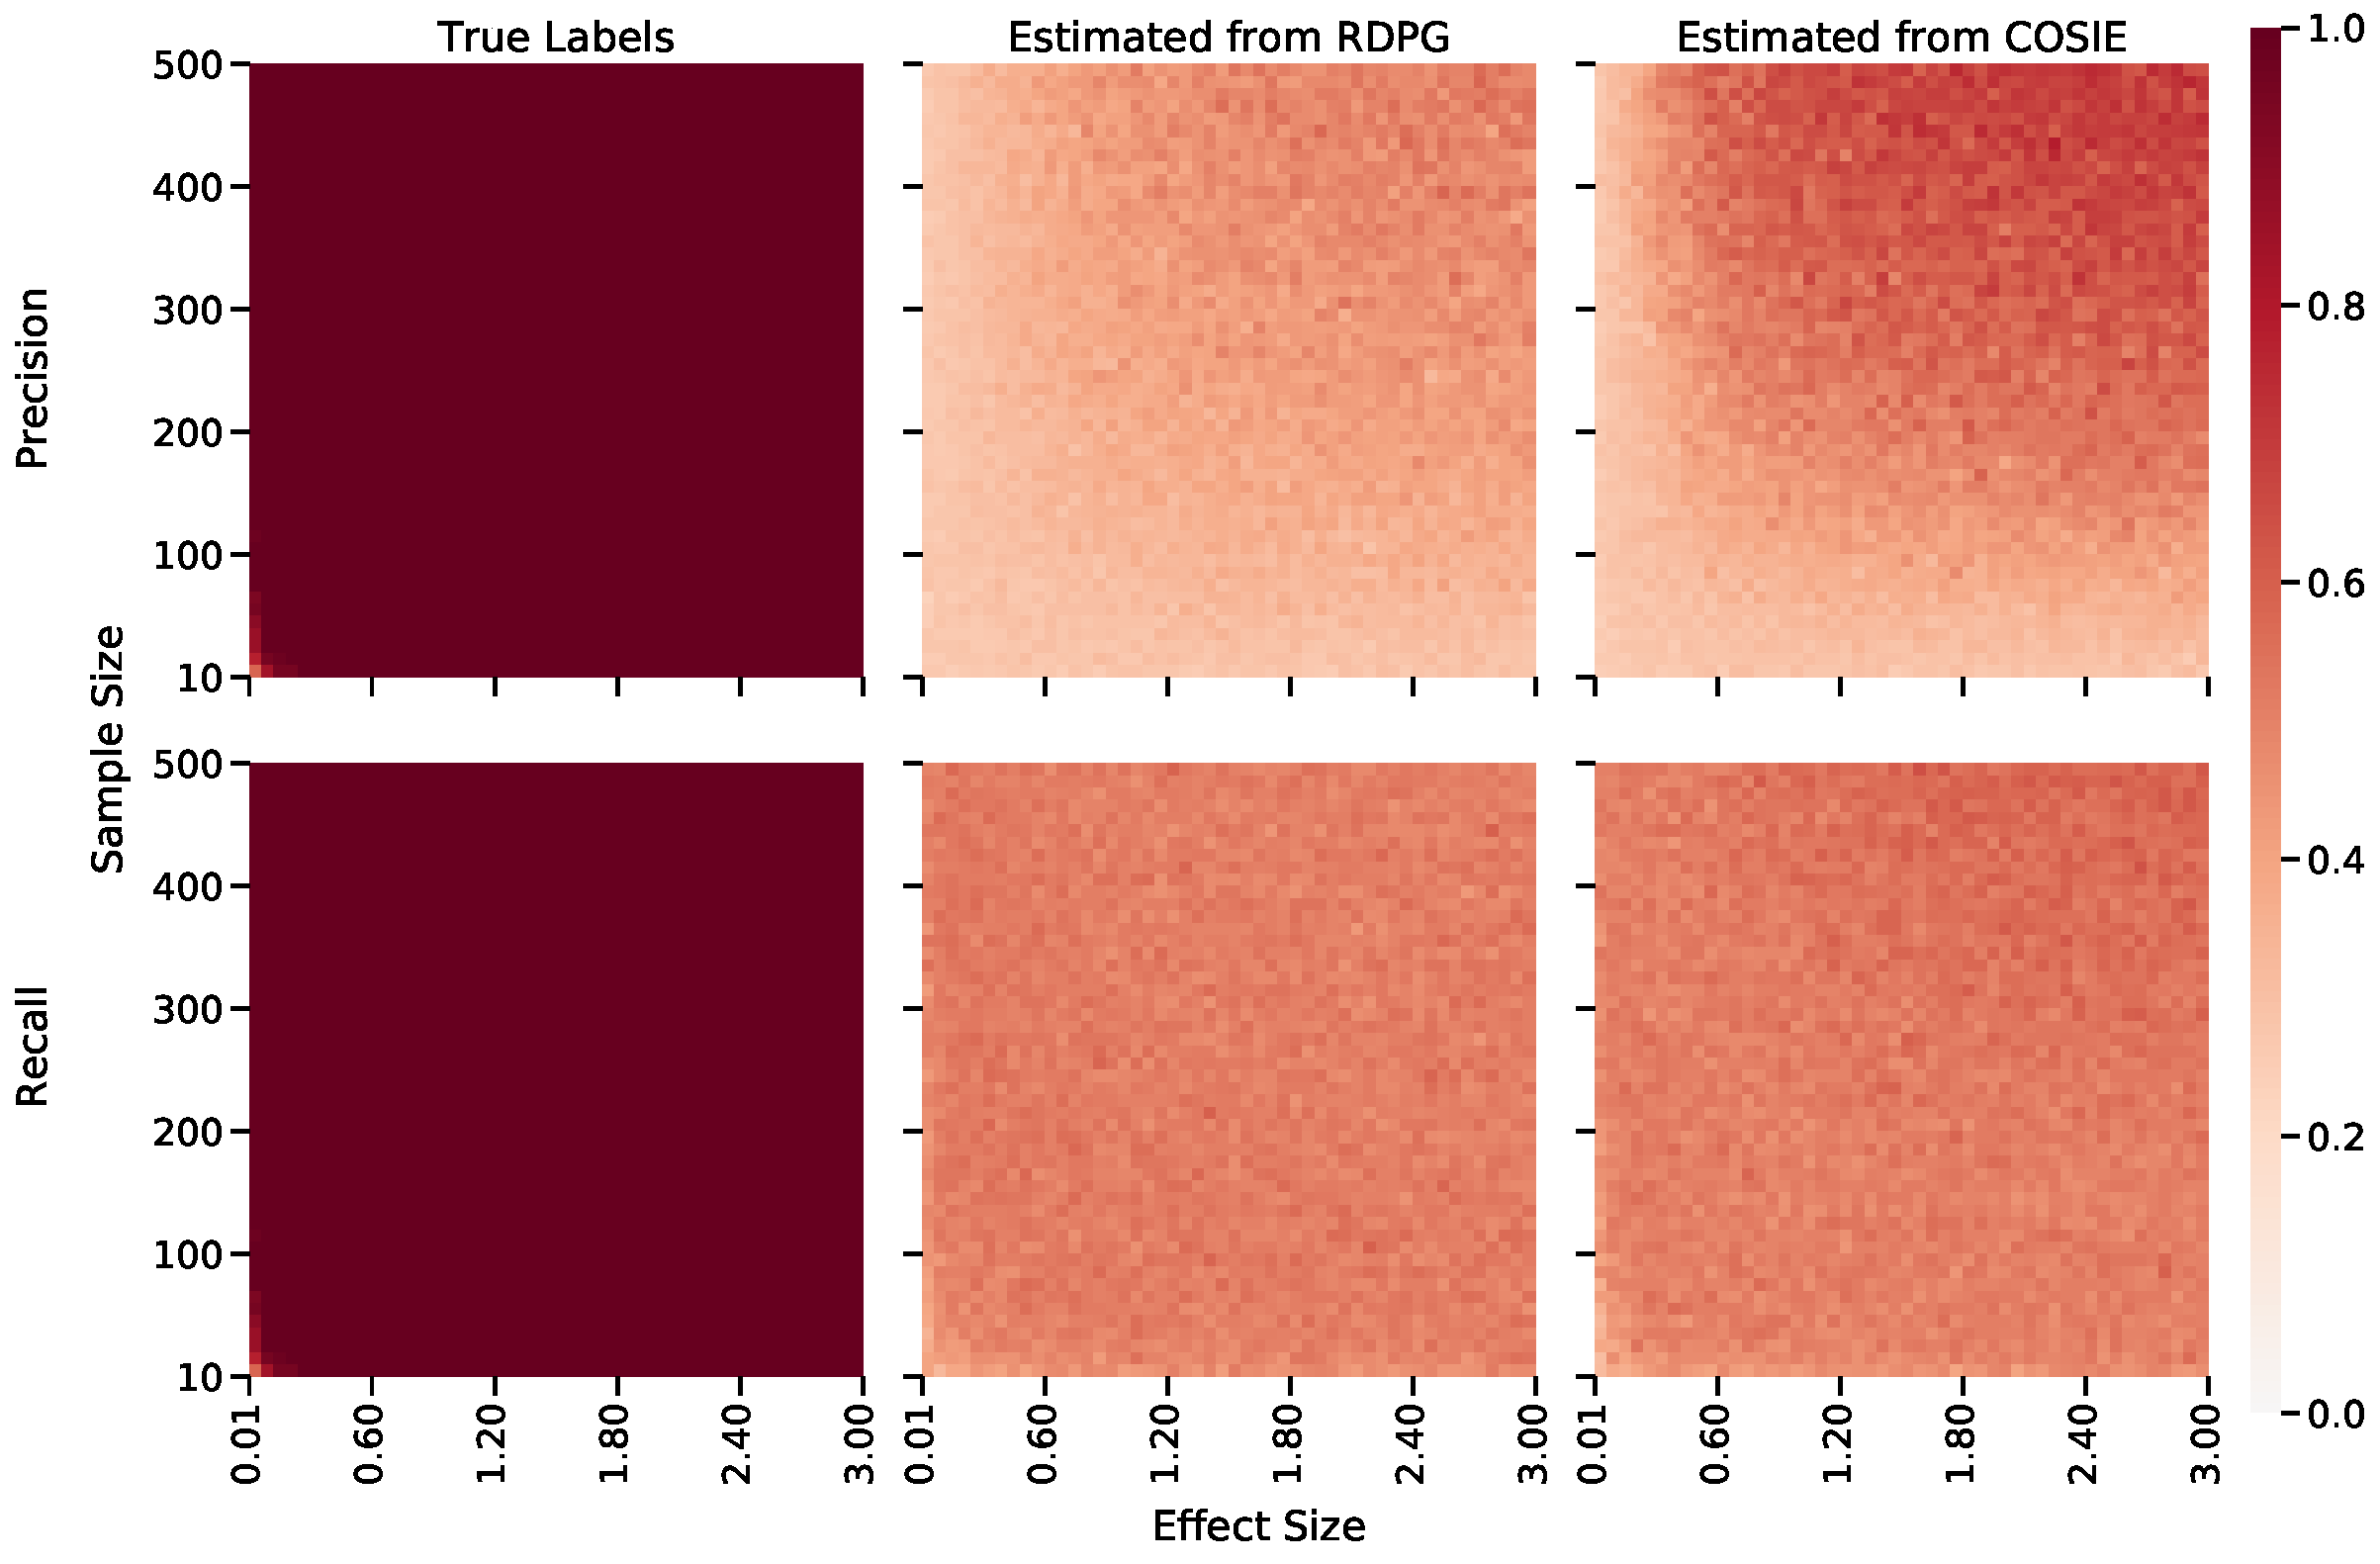
\includegraphics[width=.9\textwidth]{figures/exp4_vars_final.pdf}
    \caption{Precision \textit{(top row)} and recall \textit{(bottom row)} for significant edges using $\ks$ test sets on of edges from within community or across communities averaged over 50 trials. Effect size (x-axis) is the difference in variances of the truncated normal distribution for $B_{1,1}$.
    \textit{(Left column)} shows the precision and recall when using known community assignments. At low sample sizes ($m =10$) and low effect size ($\phi \geq 0.12$), community wise testing results in perfect precision and recall.
    \textit{(Middle column)} shows the results for using community assignments estimated under the $\jrdpg$ model.
    \textit{(Right column)} shows the results for using community assignments estimated under the $\cosie$ model.
    Communities cannot be recovered under both $\jrdpg$ and $\cosie$ model regardless of effect size and sample size. As a result, community-wise testing result in large number of false positive edges.
    }
    \label{fig:exp4_vars}
\end{figure}

% \begin{table}
%     \caption{Empirical trustworthiness computed using functional connectomes from HCP dataset.}
%     \centering
%     \begin{tabular}{c|c|c|c|c|c|c}
%         \toprule
%         \multirow{2}{*}{Hypothesis Test} &
%           \multicolumn{2}{c}{T-test} &
%           \multicolumn{2}{c}{Mann-Whitney} &
%           \multicolumn{2}{c}{Kologrov-Smirnov} \\
%          &  Precision & Recall & Precision & Recall & Precision &  Recall\\
%         \midrule
%         Right vs Right  &   x   &   x  \\
%         Left vs Left    &   x   &   x  \\
%         Left vs Right   &   x   &   x  \\
%         \bottomrule
%     \end{tabular}
%     \label{tab:exp4_hcp}
% \end{table}


% \begin{summary}[SUMMARY POINTS]
% Higher power in testing for significant edges can be achieved by comparing sets of edges rather than individual edges using community assignments.
% When community assignment must be estimated, both $\jrdpg$ and $\cosie$ models are appropriate when the edge distribution is different in means. However, both models are not useful when the edge distribution is different in variances.
% \end{summary}


